\documentclass[a4paper, 11pt]{article}
\usepackage{comment} % enables the use of multi-line comments (\ifx \fi) 
\usepackage{lipsum} %This package just generates Lorem Ipsum filler text. 
\usepackage{fullpage} % changes the margin
\usepackage{graphicx}
\usepackage{cellspace}
\setlength\cellspacetoplimit{4pt}
\setlength\cellspacebottomlimit{4pt}

\usepackage{titlesec}
\setcounter{secnumdepth}{4}

\newcommand\cincludegraphics[2][]{\raisebox{-0.3\height}{\includegraphics[#1]{#2}}}



\setlength{\parindent}{4em}
\setlength{\parskip}{1em}
\renewcommand{\baselinestretch}{1.25}

\begin{document}
%Header-Make sure you update this information!!!!
\noindent
\large\textbf{Data Visualisation Report} \hfill \textbf{Antonio Gargaro} \\
\normalsize F21DV \\
Prof. Mike Chantler  \hfill Due Date: 19/11/18  \\

\tableofcontents
\newpage

\section{Executive Summary}
% MAX 1 PAGE
% This section concisely describes goals for the project and major findings and lessons learnt
The development of a dashboard to display concise topic model data intuitively to represent rankings against word count for `Unit of Assessments', geographical focus of these units, and the weighting of the top three word collections per unit. Originally, the data provided was separate and would require users a lot of time to research and gather each document. Analysis of each document is another encumbering task in of itself. Displaying relations clearly between this data is the aim of this project.

Utilising `d3.js' and the examples provided by Mike Chantler, Mike Bostock and other `blo.cks.org' authors allows for a clear resolution towards representing this data. Specifically, licensed code was modified within the bounds of the specified license, where each source file has descriptor headings for this. Most source files are based off of Mike Chantler's work. The need to quickly filter through nested data of institutions requires the power of d3 and JavaScript to carry out data manipulation and graph these data points meaningfully in a web browser.

I find that this is possible by following the `General Update Pattern' described by Chantler and Bostock. This allows for the reuse and addition of data with efficiency to ensure an optimal experience. There is many methods provided by the d3 library to display this data in intuitive and clear ways. I ultimately decided on a sunburst for navigation, a scatter plot for comparisons and a force-directed graph for relations and comparisons.

Ultimately, d3 provides a large set of tools to complete this project. This is apparent with the ability to modify all aspects of chart generation, the ability to select specific elements already displayed and modify them, as well as the possibility of moving objects across the screen to provide an interactive experience.

\newpage
\section{Interface Design: Rationale \& Critical Review}

A large sunburst displaying all institutions allows for quick access to any specific one. A `breadcrumb' trail allows the user to keep track of where they are in this hierarchy, a legend gives a quick reference about which region matches to what colour, and an interactive map displaying what town is represented by each slice. This displays a clear navigational hierarchy for the DoR user to select specific regions, towns or institutions, while understanding what area of the UK he is searching in. 

A scatter plot graph represents all document topics one of the selected institutions contains. The `4* Rating' is plotted against the word count for each document. This allows the DoR to easily identify which documents have a high ranking and how it correlates with the word count. The easy visualisation of the plotted points displays each documents ranking very clearly. The comparison of two topics can be easily distinguished from this graph by sorting between `Environment' and `Outputs' data, aiding a DoR user.

Finally, a force-directed layout (Linked nodes) represents the analysis of a selected topic by representing the top three word combinations in a tree-like structure. The benefits of this structure allow for multiple topics to be appended onto the same institution's root node. This allows the building of a `map' to compare each weighting of the topics weights. Furthermore, the addition of more than one institution can be used as to compare the topic weights of each institution's weighting. All weightings displayed are relative to the current root node it is in. For example, if you added three different topics, the root node would add up to 100 percent. This allows for analysis of topic weightings relative to other topics by the same university.


\section{Interface Design: Layouts \& Interactivity}
\subsection{List of Layouts}
%This should use a table to list the layouts (one row per layout). The first column will contain small images of the layouts, the second column will contain short descriptions of the data used, while the third will describe how any changes to the displayed data are indicated to the user (e.g. use of transitions etc.).

\begin{center}
 \begin{tabular}{||c|p{0.3\linewidth}|p{0.3\linewidth}||} 
 \hline
 Layout Image & Data Description & Changes \\ [0.5ex] 
 \hline\hline
 \raisebox{-\totalheight}{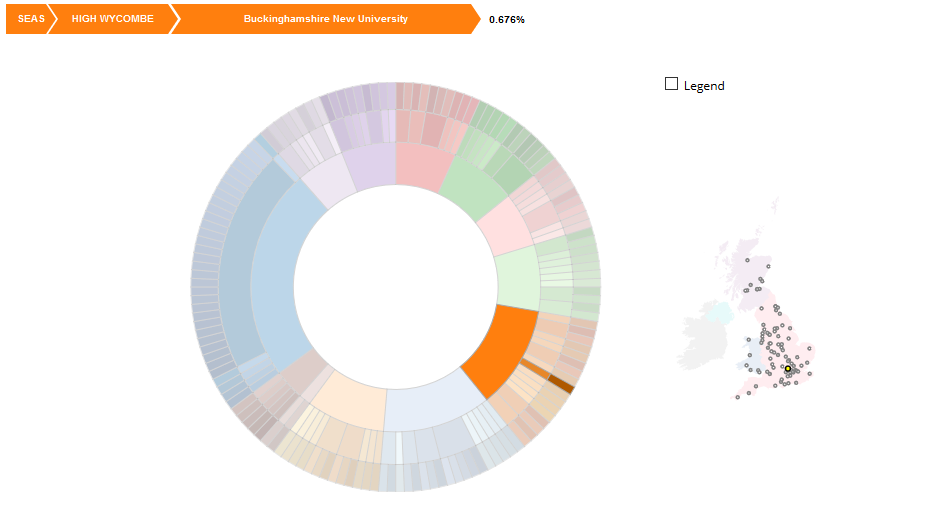
\includegraphics[width=0.3\textwidth]{imgs/Layout_SB.PNG}} 
 & This layout uses the `d3 nest' functionality with the first depth keyed to regions, the second depth keyed to towns and the third depth keyed to institutions. The `bread crumbs' and toggable legend use this data. The smaller UK map layout takes in a data set for towns \textbf{only}.
 & No data explicitly changes on the sunburst, however, selecting a town or region zooms it towards the root node and only its descendants are displayed as slices. The `bread crumb' trail has no transitions as to be responsive to mouse overs.
 \\ 
 \hline
 \raisebox{-\totalheight}{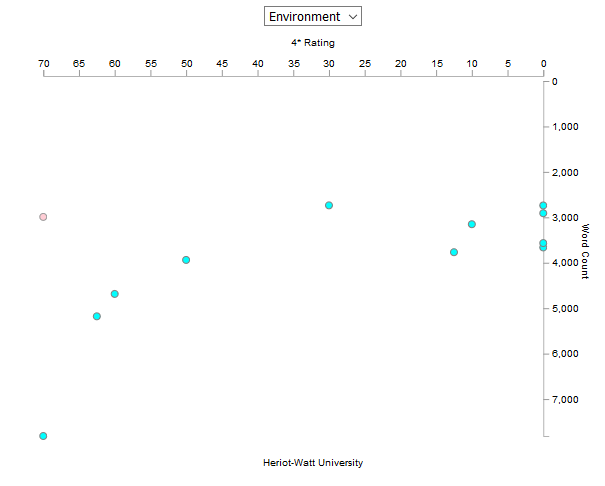
\includegraphics[width=0.3\textwidth]{imgs/Layout_SC.PNG}} 
 & This layout passes in all documents associated with a institution. This plots each point by the unique `UoAString with appended submission letters'. 
 & Topics that exist in the new selected institution change from cyan to green and move to their new location. Removed topics turn grey with half opacity and move to the bottom right corner and disappear. New topics move in from the top left corner. 
 \\
 \hline
 \raisebox{-\totalheight}{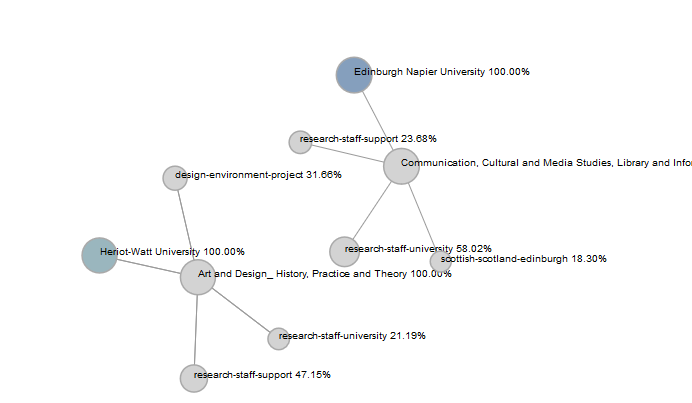
\includegraphics[width=0.3\textwidth]{imgs/Layout_NL.PNG}} 
 & This layout appends documents and refactors them into nodes with my custom addNode function. This is necessary due to how this type of graph works. It must be able to generate links between these nodes and understand their links in a flat data set. 
 & The addition of nodes move in from the top left corner and join onto existing root nodes, or make their own ones. Removal of any node fades the node and all its children out. 
 \\ [1ex] 
 \hline
\end{tabular}
\end{center}

\newpage
\subsection{Interaction between Layouts}
%This section will use images, arrows and short textual descriptions to describe the interactions between charts. Short narratives describing the rationale for these interactions should be provided.
\subsubsection{Sunburst Contained Interaction}
\begin{figure}[hbt!]
	\centering
      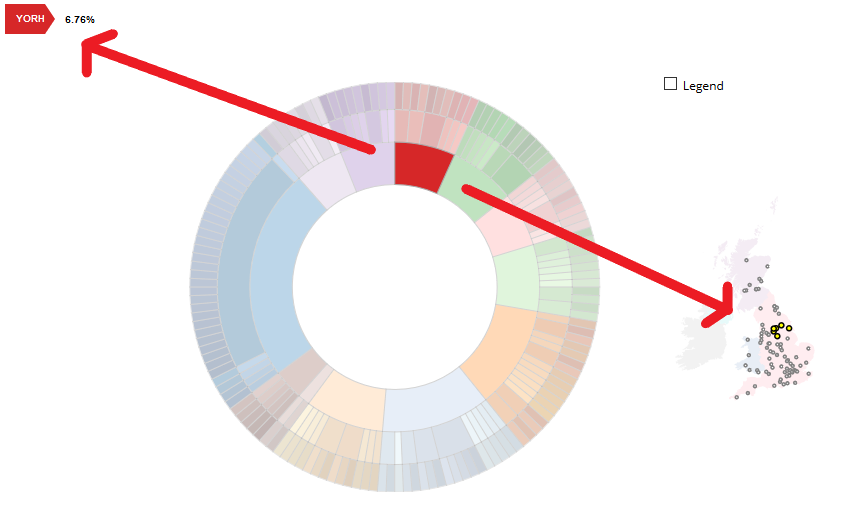
\includegraphics[width=0.6\textwidth]{imgs/sb_int/Region_select.png} \\
	\caption{Sunburst Map Highlight and Bread Crumb Trail: 
	\textit{(a)} Mouse over region highlights all towns in region on the map
	\textit{(b)} Mouse over anything displays hierarchy bread crumb trail}
	\label{fig:sb_con:reg_bread}
          \noindent\makebox[\linewidth]{\rule{\textwidth}{0.4pt}}
\end{figure}

\noindent Figure \ref{fig:sb_con:reg_bread}.a shows all towns within that region highlighted on the UK map, to represent their locations in a familiar map form. This can be used by the DoR to quickly identify where in the UK they are navigating through.

\noindent Figure \ref{fig:sb_con:reg_bread}.b shows the start of a bread crumb trail that shows the path through the descendants of the hierarchy navigation. This allows the DoR to keep track of the route he is currently navigating through.
\\

\begin{figure}[hbt!]
	\centering
      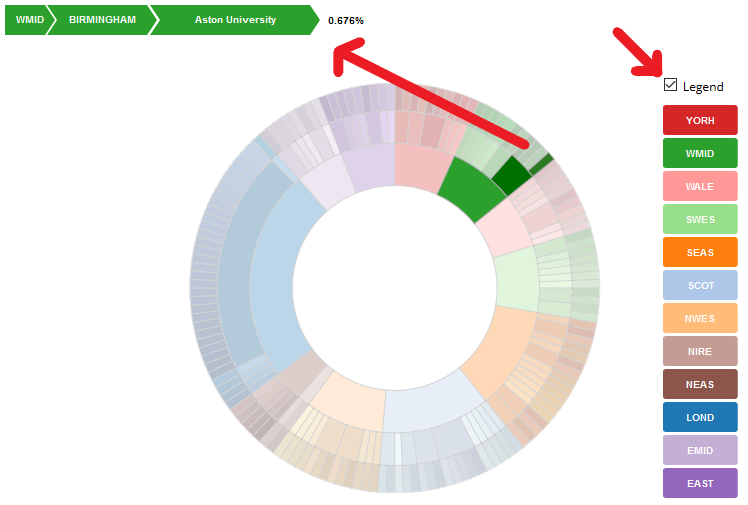
\includegraphics[width=0.5\textwidth]{imgs/sb_int/Legend_Toggle_Bread.png} \\
	\caption{Sunburst Legend Toggle: 
	\textit{(a)} Toggle checkbox to swap map with colour legend
	\textit{(b)} Mouse over anything displays hierarchy bread crumb trail}
    \label{fig:sb_con:legend_toggle_bread}
     \noindent\makebox[\linewidth]{\rule{\textwidth}{0.4pt}}
\end{figure}

\noindent Figure \ref{fig:sb_con:legend_toggle_bread}.a swaps the UK map out with a legend. This allows the DoR to also identify which region belongs to what colour. An important point is that each descendant of a region corresponds with a darker colour from the region.

\noindent Figure \ref{fig:sb_con:legend_toggle_bread}.b is similar to figure \ref{fig:sb_con:reg_bread}.b. See example above.



\begin{figure}[hbt!]
	\centering
      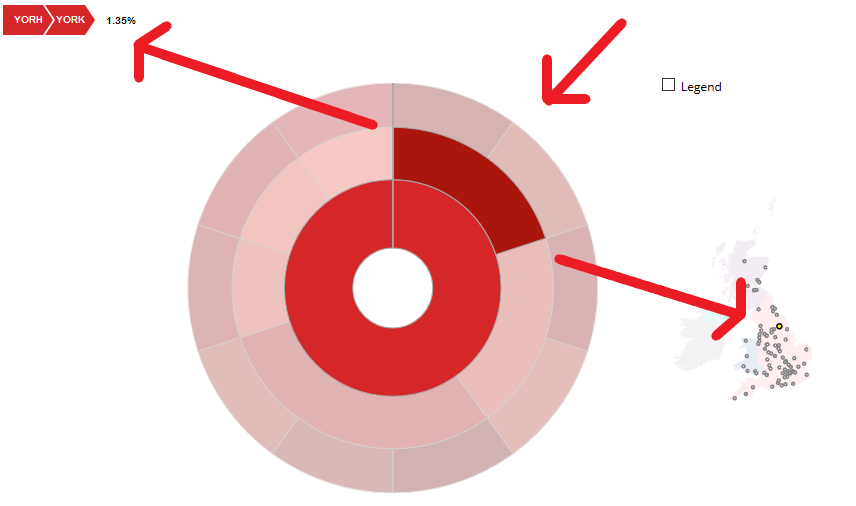
\includegraphics[width=0.6\textwidth]{imgs/sb_int/zoomable_sb.png} \\
	\caption{Sunburst Zoomable: 
	\textit{(a)} Left-click on any region or town to place it as root node}
    \label{fig:sb_con:zoomable_sb}
     \noindent\makebox[\linewidth]{\rule{\textwidth}{0.4pt}}
\end{figure}

\noindent Figure \ref{fig:sb_con:zoomable_sb}.a zooms the sunburst by selecting a region or town. This allows the DoR to filter the sunburst and focus on institutions in specific geographical areas. The UK map will only show specific towns in that region when mousing over the sunburst.

\newpage
\subsubsection{Scatter Plot Contained Interaction}
\begin{figure}[hbt!]
	\centering
      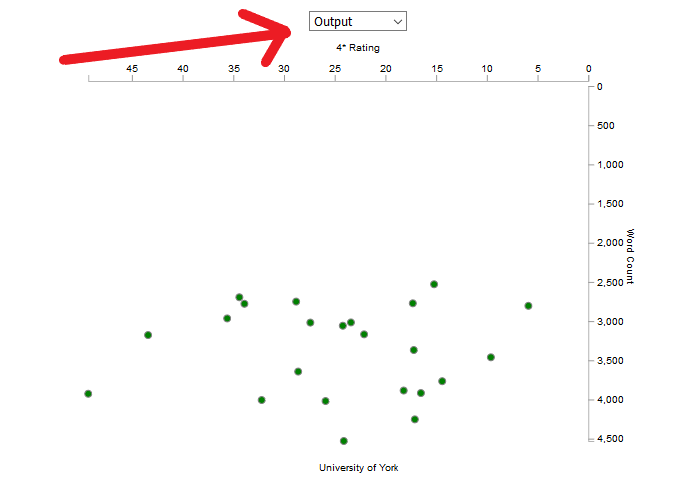
\includegraphics[width=0.6\textwidth]{imgs/sp_int/change_data.png} \\
	\caption{Scatter Plot Change Data: 
	\textit{(a)} Swap between Environment and Output}
    \label{fig:sp_con:swap_data}
     \noindent\makebox[\linewidth]{\rule{\textwidth}{0.4pt}}
\end{figure}

\noindent Figure \ref{fig:sp_con:swap_data}.a allows the swapping of 4* rating data between environment and output. This allows the DoR to compare against the specific types of rating data, giving insights of the various different types of ratings.


\subsubsection{Linked Nodes Contained Interaction}
\begin{figure}[hbt!]
	\centering
      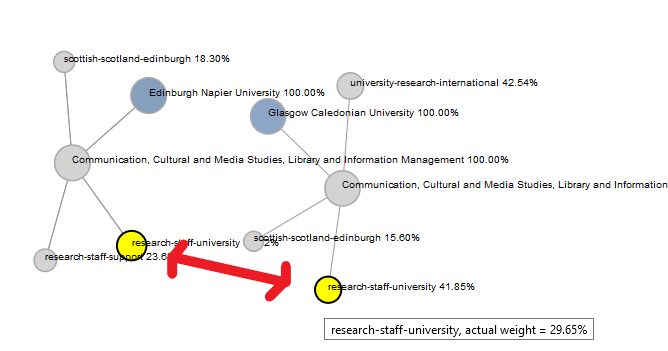
\includegraphics[width=0.6\textwidth]{imgs/ln_int/topic_weight_highlight.png} \\
	\caption{Linked Node Highlights: 
	\textit{(a)} Highlight common word combinations between topics}
    \label{fig:lp_con:common_topic_words}
     \noindent\makebox[\linewidth]{\rule{\textwidth}{0.4pt}}
\end{figure}

\noindent Figure \ref{fig:lp_con:common_topic_words}.a highlights word collections between all the topics. This is useful for the DoR as he may analyse a unit of assessment from multiple institutions, like the example above. This allows these topic words and weightings to be easily identifiable, allowing comparison of relative and actual topic weightings. This can be used with multiple institutions. \\


\begin{figure}[hbt!]
	\centering
      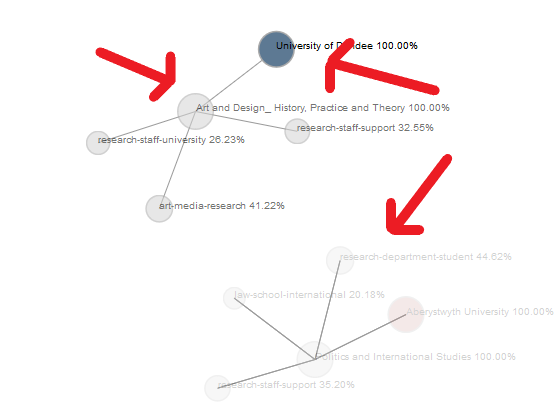
\includegraphics[width=0.6\textwidth]{imgs/ln_int/remove_nodes.png} \\
	\caption{Linked Node Highlights: 
	\textit{(a)} Removal of unit and child nodes while institution remains.
	\textit{(b} Removal of all nodes.}
    \label{fig:lp_con:remove_nodes}
     \noindent\makebox[\linewidth]{\rule{\textwidth}{0.4pt}}
\end{figure}

\noindent Figure \ref{fig:lp_con:remove_nodes}.a shows the right-click interaction to remove a unit node and all children from the linked node graph. Figure \ref{fig:lp_con:remove_nodes}.b shows the removal of an institution node. This is helpful for a DoR after no longer requiring a certain topic or institution.


\subsubsection{Scatter Plot to Sunburst Interaction}
\begin{figure}[hbt!]
	\centering
      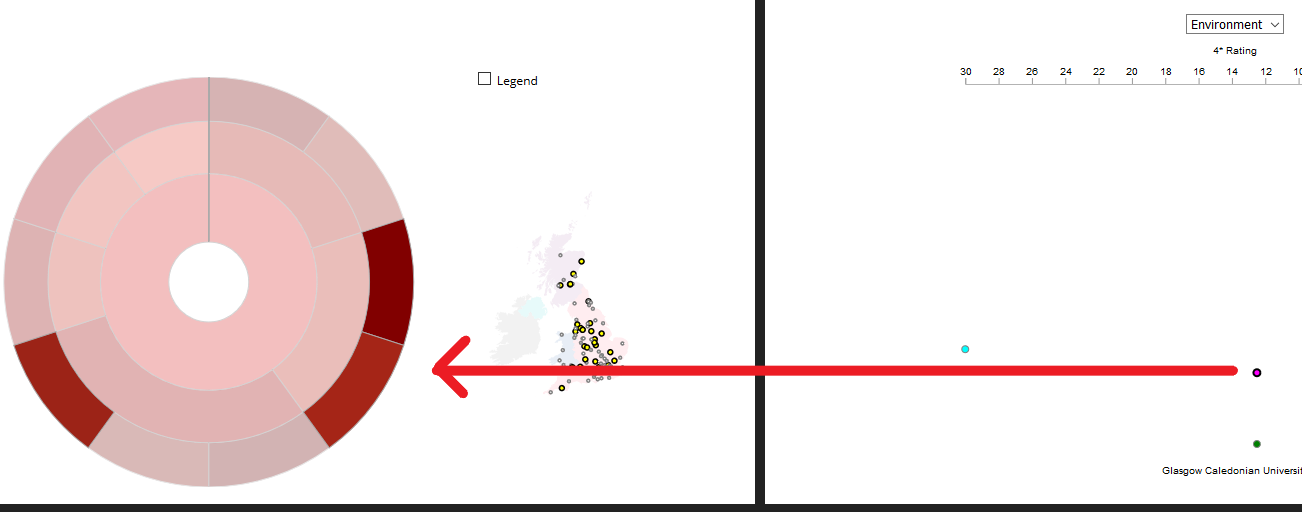
\includegraphics[width=0.6\textwidth]{imgs/sc_sb_int/select_UoA_and_compare.png} \\
	\caption{Scatter Plot Selection \& Comparison: 
	\textit{(a)} Right-click on a unit of assessment highlights it is selected.}
    \label{fig:sc_sb_int:uoa_select}
    \noindent\makebox[\linewidth]{\rule{\textwidth}{0.4pt}}
\end{figure}


\noindent Figure \ref{fig:sc_sb_int:uoa_select}.a requires a right-click to highlight a point in magenta and disables all other interactions with that point. This also freezes the sunburst to display what institutions have the selected unit of assessment. Now selecting an institution from the sunburst will only pull the selected topics data onto the scatter plot to allow for easy comparison. After performing this action will reset the unit selection. This is useful for the DoR to allow for quick reference to what institutions have a document for the selected unit. This can provide clear comparisons of their 4* ratings.


\subsubsection{Linked Node to Sunburst Interaction}
\begin{figure}[hbt!]
	\centering
      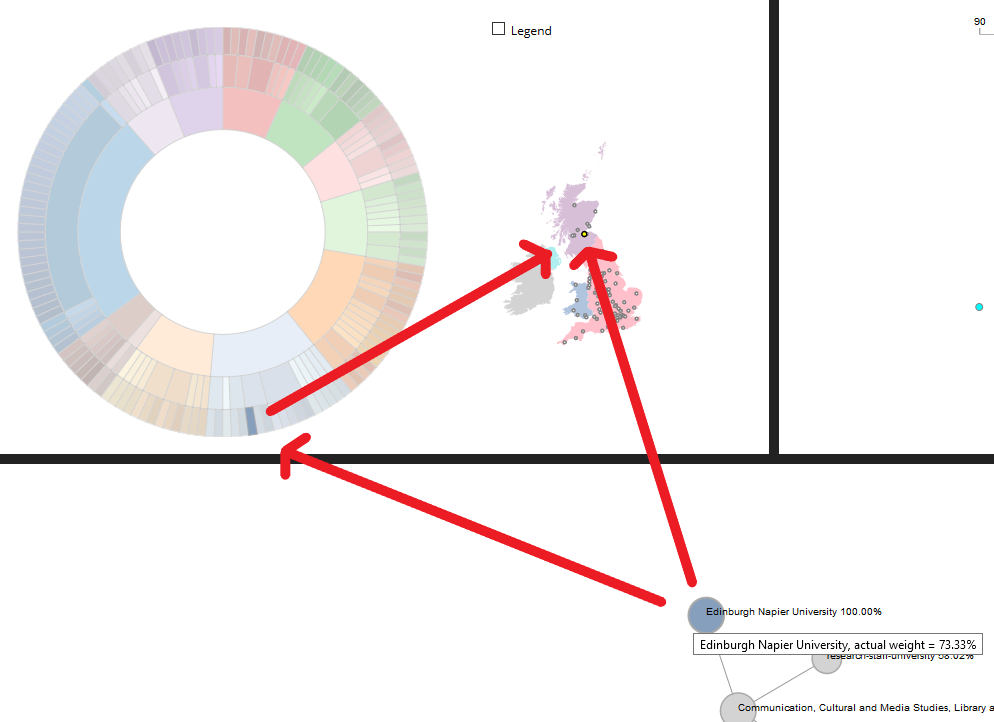
\includegraphics[width=0.6\textwidth]{imgs/sb_ln_int/LN_SB_Institute_map_highlight.png} \\
	\caption{Linked Node Highlights Institution: 
	\textit{(a)} Highlight institution on sunburst and town on the map.}
    \label{fig:ln_sb_int:institution_town_highlight}
     \noindent\makebox[\linewidth]{\rule{\textwidth}{0.4pt}}
\end{figure}

\noindent Figure \ref{fig:ln_sb_int:institution_town_highlight}.a highlights the current moused over institution on the sunburst, and highlights its location on the map. This is useful for the DoR to easily identify where on the sunburst the institution is positioned, while also feeding back its geographical location.


\subsubsection{Sunburst, Scatter Plot and Linked Node Interactions}
\begin{figure}[hbt!]
	\centering
      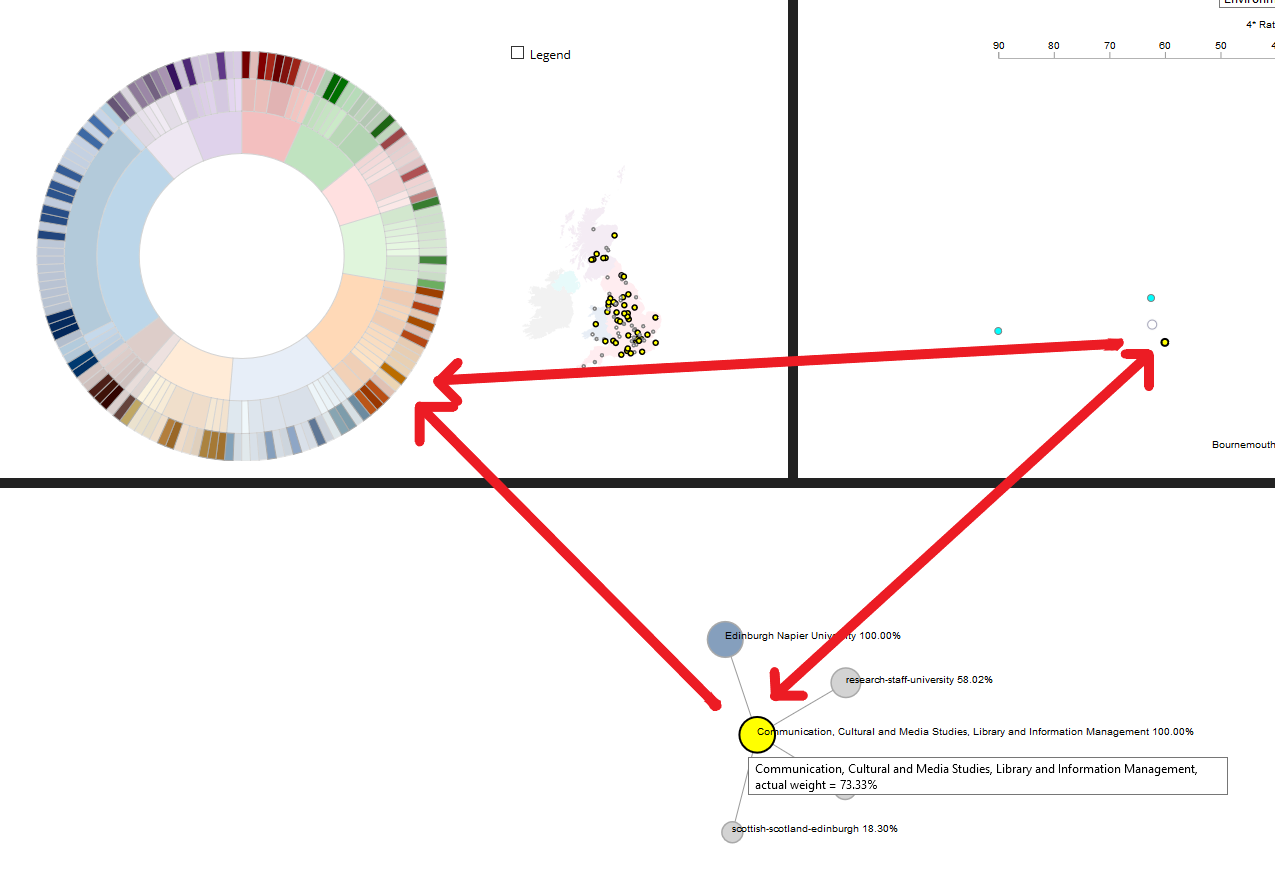
\includegraphics[width=0.42\textwidth]{imgs/sb_sc_ln_int/3_way_topic_highlight.png} \\
	\caption{Unit of Assessment Highlights: 
	\textit{(a)} Mouse over on Linked Node unit highlights same unit on scatter plot and every institution that contains that unit on the sunburst.
	\textit{(b)} Same as \ref{fig:sb_sc_ln_int:3_way_topic_highlight}.a but mouse over on scatter plot point highlights same unit on linked node.}
    \label{fig:sb_sc_ln_int:3_way_topic_highlight}
     \noindent\makebox[\linewidth]{\rule{\textwidth}{0.4pt}}
\end{figure}

\noindent Figure \ref{fig:sb_sc_ln_int:3_way_topic_highlight}.a and \ref{fig:sb_sc_ln_int:3_way_topic_highlight}.b highlights where this unit of assessment is present on the scatter plot or the linked node respectively. Mousing over a unit on either graph displays what institution this unit is present in on the sunburst. This is useful for the DoR as it shows quickly what institution has a document based on that unit. It also allows to quick display where each document is on the scatter plot and linked node graph. This can especially be useful, for example, to quickly locate where the the current unit moused over on the linked node graph is on the scatter plot graph. Similarly, this can check if the unit moused over on the scatter plot is currently present in the linked node graph. \\

\begin{figure}[hbt!]
	\centering
      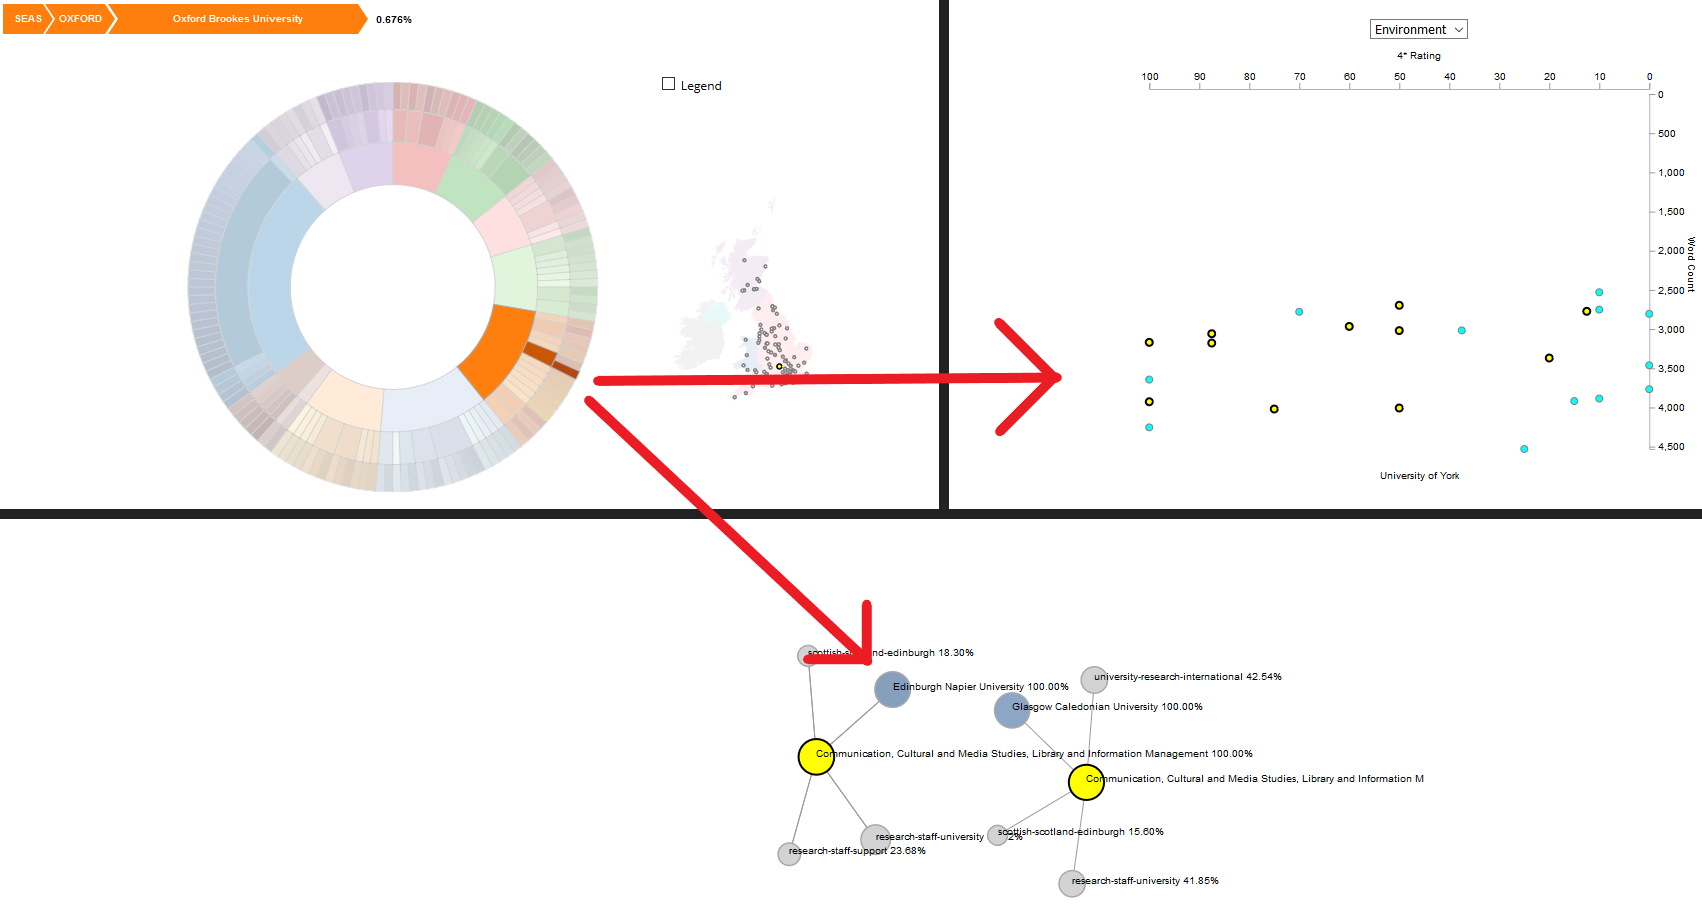
\includegraphics[width=0.5\textwidth]{imgs/sb_sc_ln_int/topics_in_current_and_in_highlighted.png} \\
	\caption{All Unit of Assessment Highlights: 
	\textit{(a)} Mouse over on sunburst institution highlights all the units which are also currently present on the scatter plot and linked node graph.}
    \label{fig:sb_sc_ln_int:topics_in_cur_mouse}
     \noindent\makebox[\linewidth]{\rule{\textwidth}{0.4pt}}
\end{figure}

\noindent Figure \ref{fig:sb_sc_ln_int:topics_in_cur_mouse}.a shows that when mousing over an institution on the sunburst, what units that are currently being represented in the scatter plot and linked node graphs are also present in that institution. This is particularly helpful for the DoR as to confirm that another unit they are looking for has the specific unit they are comparing.



\newpage
\section{Software Design}
\subsection{Design overview}
% (one page max) This should provide a diagram and short associated narrative describing the top-level structure of your design (i.e. how you have split the design up into the various source files and what their runtime equivalents communicate with each other).

\begin{center}
 \begin{tabular}{||c|p{0.65\linewidth}||} 
 \hline
 Project Stucture & Description \\ [0.5ex] 
 \hline\hline
 \raisebox{-\totalheight}{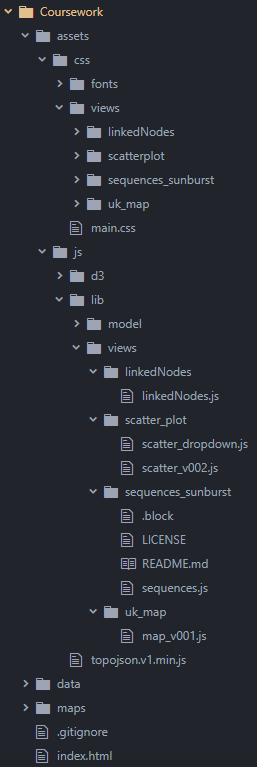
\includegraphics[width=0.3\textwidth]{imgs/project_struct/project_structure.png}} 
 & 
 This project is based off a modular design. All charts are within the \textbf{`./js/lib/views/'} and matching to their own folder. These files are imported from the \textbf{`./index.html'} file. This file corresponds with the initialisation function presented by Chantler. This file also contains communal functions that each modular code imported can utilise. These functions work with variables assigned to the modular charts and are used to render data and display interactions.
 
 Each chart also has its own corresponding css file in \textbf{`./css/views/'} with their own folder. This allows to easily change specific highlighting designs, and is also imported into the \textbf{`./index.html'} file.
 \\ 
 \hline
\end{tabular}
\end{center}


\newpage
\subsection{Use of Design Patterns}
% This section should briefly describe any software design patterns that you have used. Each design pattern (together with a critical analysis of what their advantages and disadvantages were for your project) should be described in their own, short, numbered subsection (4.2.1, 4.2.2 … etc.)
\subsubsection{Function Class}
A prevalent software design pattern for this project was a function class. This is essentially a function imitating a class definition. This has it's advantages such as providing information hiding techniques and assigning variables locally for that class. This means data cannot accidentally be modified else where in this project. Another benefit of this allows for overrides of specific functions of variables when explicitly stated. For example, updating an accessor function when changing data on my scatter plot chart (See figure \ref{fig:sc_sb_int:uoa_select}). This also allowed for function chaining when continually returning an object from each public method.

This has disadvantages however, by not allowing to return data explicitly when chaining multiple functions. This required the use of d3's select function to get data from DOM elements instead, which is not as efficient as direct access to a basic `getter' function.

\subsubsection{Global Functions}
Assigning global helper functions in the main \textbf{`./index.html'} allowed for cleaner syntax and less code repetition between charts. An example of this is `resetting' charts after modifying specific elements. This function quickly returned interacted elements back to their default state with one function call. This reduced development time greatly without constant implementation.

\subsubsection{Function Callbacks}
This project has numerous amounts of function callbacks to handle functionality cleanly. This is also beneficial for changing what these functions do on the fly. This was useful in my project when I swap my x-axis data plots from `environment' to `output'. It was also beneficial for disabling mouse click and mouse over functionality when selecting a topic from my scatter plot.




\section{Original contribution made by the student}
\subsection{Highlights} 
% This section should briefly identify and highlight anything that you feel particularly proud of that you would like to bring to the attention of the examiners. 
\subsubsection{Linked Node Implementation}
I am particularly proud of this chart design as I implemented a node creation function that fitted document data into the flat data set required by this layout (See \textbf{`addNodes()'} in \textbf{`linkedNode.js'}). I also implemented traversal functions to update node weights on addition or deletion, delete specific nodes and delete all their children nodes (See \textbf{`removeNodeAndChildren()'} and \textbf{`updateWeights()'} in \textbf{`linkedNode.js'}).

\subsubsection{Scatter Plot Selection Implementation}
I implemented a point selection function on the scatter plot graph to allow comparison of two or more units when selecting another institution. This kept the current point in the graph and filtered the new incoming data to only allow the selected unit (See \textbf{`checkAnySelected()'} and \textbf{`rightClickFunction()'} in \textbf{`sequences.js'})..

\subsubsection{Bread Crumb Trail Scale to Words}
I modified the bread crumb implementation to allow the sizing to fit the displayed word when it is rendered with. This did not come with the original implementation of this sunburst (See \textbf{`updateBreadcrumbs()'} in \textbf{`sequences.js'}).

\subsection{File by File description}
% A subsection should be provided for each of your application’s software source files (e.g. 5.2.1, 5.2.2, etc,). The subsections should have the same name as the source files. They should start with a table indicating the percentage contributions of the sources, and if applicable, the source of the code and its licence as shown in the example below:


\subsubsection{index.html}
\begin{center}
 \begin{tabular}{||p{0.15\textwidth}|p{0.15\textwidth}|p{0.15\textwidth}|p{0.15\textwidth}|p{0.15\textwidth}||} 
 \hline
 Contribution by student & Contribution from course & contribution from 3rd party & Source & Licence 
 \\
 \hline
 40\% & 60\% & 0\% &  &
 \\
 \hline
\end{tabular}
\end{center}
I implemented many extra interaction functions for selection towards the bottom of the file to ease development.

\subsubsection{sequences.js}
\begin{center}
 \begin{tabular}{||p{0.15\textwidth}|p{0.15\textwidth}|p{0.15\textwidth}|p{0.15\textwidth}|p{0.15\textwidth}||} 
 \hline
 Contribution by student & Contribution from course & contribution from 3rd party & Source & Licence 
 \\
 \hline
 43\% & 10\% & 47\% & Block 766f8f6d31f645 c39f488a0befa 1e3c8, Block 1a3f8e44cdcb3 054121dfd991f 59fbc2 & Apache 2.0, GNU General Public License, version 3
 \\
 \hline
\end{tabular}
\end{center}
I heavily modified the original file to correspond with the same setup used in the course. This allows me to understand how this view works as well as showing understanding of methods learned during this course. I also implemented the zooming function provided by the second source. I originally gave my contribution as 40\%, the course as 10\% and sources as 50\%, but I also implemented a toggle feature for the map in this file so that is why the contribution is higher than my original 40\% rating.


\subsubsection{scatter\_v002.js}
\begin{center}
 \begin{tabular}{||p{0.15\textwidth}|p{0.15\textwidth}|p{0.15\textwidth}|p{0.15\textwidth}|p{0.15\textwidth}||} 
 \hline
 Contribution by student & Contribution from course & contribution from 3rd party & Source & Licence 
 \\
 \hline
 35\% & 65\% & 0\% & & 
 \\
 \hline
\end{tabular}
\end{center}
I implemented extra functionality, such as point selection for units. I also added in extra labels for the axises and bottom of the grid. I swapped the axis orientations from left and bottom to right and top. I also added the drop down bar from another lab, however it is part of the course.

\subsubsection{scatter\_dropdown.js}
\begin{center}
 \begin{tabular}{||p{0.15\textwidth}|p{0.15\textwidth}|p{0.15\textwidth}|p{0.15\textwidth}|p{0.15\textwidth}||} 
 \hline
 Contribution by student & Contribution from course & contribution from 3rd party & Source & Licence 
 \\
 \hline
 0\% & 100\% & 0\% & & 
 \\
 \hline
\end{tabular}
\end{center}


\subsubsection{linkedNodes.js}
\begin{center}
 \begin{tabular}{||p{0.15\textwidth}|p{0.15\textwidth}|p{0.15\textwidth}|p{0.15\textwidth}|p{0.15\textwidth}||} 
 \hline
 Contribution by student & Contribution from course & contribution from 3rd party & Source & Licence 
 \\
 \hline
 65\% & 10\% & 25\% & Block 1129492, Block 6c282b65246f8 f46bb55aadc32 2db709 &  GNU General Public License, version 3
 \\
 \hline
\end{tabular}
\end{center}
I heavily modified the original file to correspond with the same setup used in the course. This allows me to understand how this view works as well as showing understanding of methods learned during this course. I also modified the code to implement node creating when new documents were added in. I also added methods to manipulate nodes, such as modify the weight, scaling them correctly, deletion of nodes and there children and addition of labels onto nodes.


\subsubsection{map\_v001.js}
\begin{center}
 \begin{tabular}{||p{0.15\textwidth}|p{0.15\textwidth}|p{0.15\textwidth}|p{0.15\textwidth}|p{0.15\textwidth}||} 
 \hline
 Contribution by student & Contribution from course & contribution from 3rd party & Source & Licence 
 \\
 \hline
 2\% & 98\% & 0\% &  & 
 \\
 \hline
\end{tabular}
\end{center}
I only modified the scaling of the map for this file.



%This should be followed by a short description of the student’s contribution to the module (source file). If the student’s contribution to a particular source file is 0\% then,  no narrative is required.

\newpage
\section*{Source code listings}

\subsection{index.html}

\begin{verbatim}

<!--------------------------------------------------------------------

   Module: main html file for Data visualization coursework

   Author: Antonio Gargaro

   What it does:
  	Constructs all module parts of coursework in here

---------------------------------------------------------------------->

<!doctype html>
<html lang="en">

<head>
  <meta charset="utf-8">
  <title>Data visualization Dashboard - Coursework</title>
  <meta name="description" content="">
  <meta name="viewport" content="width=device-width, initial-scale=1, shrink-to-fit=no">

  <link rel="manifest" href="site.webmanifest">
  <link rel="apple-touch-icon" href="icon.png">

  <link rel="stylesheet" href="./assets/css/main.css">
  <!-- import views css -->
  <link rel="stylesheet" type="text/css" href="./assets/css/views/sequences_sunburst/sequences.css" />
  <link rel="stylesheet" type="text/css" href="./assets/css/views/uk_map/map-v001.css" />
  <link rel="stylesheet" type="text/css" href="./assets/css/views/scatterplot/scatterplot.css" />
  <link rel="stylesheet" type="text/css" href="./assets/css/views/linkedNodes/linkedNodes.css" />
  <link rel="stylesheet" type="text/css" href="./assets/css/fonts/OpenSans.css">

  <!-- import javascript lib dependency files -->
  <script type="text/javascript" src="./assets/js/d3/d3.v4.js"></script>
  <script type="text/javascript" src="./assets/js/lib/model/ref14model_v003.js"></script>
</head>

<body>
  <!--
  Contains the sunburst graph. This is licenced under
  apache 2.0, link available in report.
  -->
  <div class='dashboard'>

    <div class='column'>
      <div id="chart1" class="item">
        <div class="flex_row flex_nowrap">
          <div class="flex_column flex_grow">
            <div id="sequence"></div>
            <div class="flex_row align_centre">
              <div id="explanation" style="visibility: hidden;">
                <span id="percentage"></span><br /> of visits begin with this sequence of pages
              </div>
              <div id="sb1"></div>
              <div id="sidebar" class="flex_grow">
                <input type="checkbox" id="togglelegend" autocomplete="off"> Legend<br />
                <div id="sb1_map" style="visibility: visible" class="map"></div>
                <div id="legend" style="visibility: hidden;"></div>
              </div>
            </div>
          </div>

        </div>
      </div>

      <div id="chart2" class="item align_centre flex_column">
        <div id="sc1_dropdown">

        </div>
        <div id="sc1" class="align_centre">

        </div>
      </div>
    </div>


    <div class='column'>
      <div id="chart3" class='item'>
        <div id="lnc1" class="align_centre">

        </div>
      </div>
    </div>

  </div>


  <!--  import views js -->
  <script type="text/javascript" src="./assets/js/lib/views/sequences_sunburst/sequences.js"></script>
  <script type="text/javascript" src="./assets/js/lib/views/uk_map/map_v001.js"></script>
  <script type="text/javascript" src="./assets/js/lib/views/scatter_plot/scatter_v002.js"></script>
  <script type="text/javascript" src="./assets/js/lib/views/scatter_plot/scatter_dropdown.js"></script>
  <script type="text/javascript" src="./assets/js/lib/views/linkedNodes/linkedNodes.js"></script>
  <script type="text/javascript" src="./assets/js/topojson.v1.min.js"></script>



  <script type="text/javascript">
    "use strict"

    var dm1 = modelConstructor()
      .addBasicTopicArrayData(false); //Create datamodel object (gives access to methods in ref14model.js etc )
    var dataModel; //shorthand for dm1.model() and declared as nasty outer block variable for easy access from console.
    var sb1; //Sunburst 1
    var map1; //UK Map1
    var sc1;
    var lnc1; //Linked Node Chart
    var countries;


    //=============== READ DATA FILES ================================
    d3.queue()
      .defer(d3.csv, "data/topics/REF2014T30TopicOrder.csv")
      .defer(d3.csv, "data/290183_REF_Contextual_table_1314_0.csv")
      .defer(d3.csv, "data/learning-providers-plus.csv")
      .defer(d3.json, "data/topics/REF2014T30Python.json")
      .defer(d3.csv, "data/REF2014_Results.csv")
      .defer(d3.json, "maps/uk.json")
      .await(initialiseApp)

    //======================== MAIN FUNCTION =================================
    //Carries out all initialization and setup
    function initialiseApp(error, ref14data, ref14context, learningProviders, jsonTopicData, REFcsvData, uk) {
      //Check data files have loaded
      if (error) {
        console.log(" there are errror with loading the data: ", error);
        return;
      }

      //Create data model
      dm1.loadData(ref14data, ref14context, learningProviders, jsonTopicData, REFcsvData);
      dataModel = dm1.model()


      //Draw the basic map
      countries = topojson.feature(uk, uk.objects.subunits).features;
      //Group REF entries by town
      var townGroups = d3.nest().key(e => e.lp.TOWN).entries(dataModel.refEntries);
      map1 = map("#sb1_map");
      map1
        .loadAndRenderMap(countries)
        .overrideTownNameAccessor(d => firstCaps(d.key));
      map1.loadAndRenderTowns(townGroups);


      //Layout and render flat data as sunburst
      var nest = d3.nest()
        .key(refEntry => refEntry.context.regionProvider)
        .sortKeys(d3.ascending) //sort a-z
        .key(refEntry => refEntry.lp.TOWN)
        .sortKeys(d3.ascending)
        .key(refEntry => refEntry["Institution name"])
        .sortKeys(d3.ascending)
        .rollup(values => values) //add rollup to campact leaves and store refEntry info
        .entries(dataModel.refEntries);
      //Load data into sunburst with rootnode
      sb1 = sunburst("#sb1")
        .loadAndRenderNestDataset(nest, "REF2014")


      //Get list of Universities to initialise
      //other graphs.
      var universities = d3.nest()
        .key(function(d) {
          return d["Institution name"];
        })
        .sortKeys(d3.ascending)
        .entries(dataModel.refEntries);
      //Mimic document object
      universities = universities.map(e => {
        return {
          data: {
            key: e.key,
            values: e.values
          }
        };
      });


      //Create scatterplot
      sc1 = scatterplot("#sc1")
        .overridesepalWidthFunction(function(e) {
          return Number(e.environment["4*"])
        }) //Use the 4* assessment as the bar size
        .overridesepalLengthFunction(function(e) {
          return Number(e.environment["WordCount"])
        })
        //Useful for updating current uni's UoA with new uni
        .overrideKeyFunction(e => e["UoAString with Multiple submission letter appended"])
        .overrideTooltipFunction(e => {
          return e["Institution name"] + ", " + e["UoAString with Multiple submission letter appended"] + ", 4* = " + e.environment["4*"];
        });
      //render scatter with first university's data
      renderUniversityData(universities[0])

      //Add scatter drop-down
      var dataSelect = d3.select('#sc1_dropdown')
        .append('select')
        .attr('id', 'sc1SelectID')
        .on('change', onSCDataChange)

      renderSCDataOptions(dataSelect); //Add choice options


      //Initialuse linked node chart
      lnc1 = linkedNodesChart("#lnc1");
      //render nodes with first university's first UoA data
      addAssessmentTop3Weights(universities[0].data.values[0]);


      //Print main dataModel object to Console
      console.log("\nFor ease of inspection: dataModel = ", dataModel)


      function firstCaps(name) {
        return name[0] + name.slice(1).toLowerCase()
      };
    }


    //========= DATA FUNCTIONS ===========//

    function renderUniversityData(d) {
      //console.log(d);
      let university = d.data.key;
      //Generate set of REF entries for this university
      var sc1Data = dataModel.refEntries
        .filter(e => e["Institution name"] == university)
        .sort(function(a, b) {
          return a["UoAString with Multiple submission letter appended"] > b["UoAString with Multiple submission letter appended"]
        })
      //Render the barchart
      sc1.loadAndRenderDataset(sc1Data);
      //console.log("SC1 = ", sc1Data);
    }

    function addAssessmentTop3Weights(document) {
      //console.log(document);
      lnc1.loadAndRenderDataset(document);
    }


    //========= INTERACTION FUNCTIONS ===========//

    function opacityClassKey(keys) {
      for (let i = 0; i < keys.length; i++) {
        d3.selectAll(".sbNodesGroup > path").each(function(d) {
          if (!d3.select(this).classed(keys[i]))
            d3.select(this).style("opacity", 0.3);
          else {
            let institution = d3.select(this).data()[0].data
            let town = institution.value[0].lp.TOWN;
            d3.select(".key--" + town.toLowerCase()).classed("highlight", true).selectAll("circle").attr("r", 2.5);
          }
        });
      }
    }

    function highlightClassKey(keys) {
      for (let i = 0; i < keys.length; i++) {
        d3.selectAll("." + keys[i]).classed("highlight", true);
      }
    }

    function unhighlightClassKey(keys) {
      for (let i = 0; i < keys.length; i++) {
        d3.selectAll("." + keys[i]).classed("highlight", false);
      }
    }

    function getKeyClasses(d) {
      let classes = d.attr("class").split(" ");
      let keys = [];

      for (let i = 0; i < classes.length; i++) {
        if (classes[i].startsWith("key--"))
          keys.push(classes[i]);
      }
      return keys;
    }

    function highlightUniversities(subject) {
      var allUnisWithSubject = dataModel.refEntries
        .filter(e => e["UoAString"] == subject).map(e => [e["Institution name"], e.lp.TOWN]);
      // Fade all the segments.
      d3.selectAll("g.sbNodesGroup path, g.mapGroup path").style("opacity", 0.3);

      for (var i = 0; i < allUnisWithSubject.length; i++) {
        var sbKey = ".key--" + (allUnisWithSubject[i][0]).replace(/[\W]+/g, "_");
        var mapKey = ".key--" + (allUnisWithSubject[i][1]).replace(/[\W]+/g, "_").toLowerCase();

        d3.select(sbKey).style("opacity", 1);
        d3.select(mapKey).classed("highlight", true).selectAll("circle").attr("r", 2.5);
      }
    }

    function resetAllhighlights() {
      resetTowns();
      resetSunburst();
      resetScatter();
      resetLinkedNode();}

    function resetLinkedNode() {
      d3.selectAll("g.nodeGroup > g.node > circle").classed("highlight", false);
    }

    function resetScatter() {
      d3.selectAll("svg.scatterplot > circle").classed("highlight", false);
    }

    function resetSunburst() {
      d3.selectAll("g.sbNodesGroup path, g.mapGroup path").style("opacity", 1);
    }

    function resetTowns() {
      d3.selectAll("g.classTown")
        .classed("highlight", false)
        .each(function(d, i) {
          var children = d3.selectAll(this.childNodes);
          children.attr("r", 1.5);
        });
    }
  </script>

</body>

</html>

    
\end{verbatim}

\newpage
\subsection{sequences.js}

\begin{verbatim}
    
/*
Note by Antonio Gargaro:
This code was available on bl.ocks.org and licenced under Apache 2.0
Author: Kerry Rodden
Date Retrieved: 19/10/2018
Link: https://bl.ocks.org/kerryrodden/766f8f6d31f645c39f488a0befa1e3c8

Implemented the zooming funcitonality with
GNU General Public License, version 3 from,
Author: David Richard's
Date Retrieved: 28/10/2018
Link: https://bl.ocks.org/denjn5/1a3f8e44cdcb3054121dfd991f59fbc2
*/

/*
Apache 2.0 Licence

Copyright 2013 Google Inc. All Rights Reserved.

Licensed under the Apache License, Version 2.0 (the "License");
you may not use this file except in compliance with the License.
You may obtain a copy of the License at

   http://www.apache.org/licenses/LICENSE-2.0

Unless required by applicable law or agreed to in writing, software
distributed under the License is distributed on an "AS IS" BASIS,
WITHOUT WARRANTIES OR CONDITIONS OF ANY KIND, either express or implied.
See the License for the specific language governing permissions and
limitations under the License.

 */

var hierarchyGraph; //The graph of objects used to represent the hierarchy
var node; // Keep track of root

function sunburst(targetDOMelement) {
  /* I modified the original file to correspond with the same
  setup used in the labs. This allows me to understand how this
  view works as well as showing understanding of methods learned
  during lectures and labs.

  This is allowed under the Apache 2.0 Licence
  */

  //Declare the main object that will be returned to the caller
  var sunburstObject = {};

  //=================== PUBLIC FUNCTIONS =========================
  //
  sunburstObject.loadAndRenderNestDataset = function(
    nestFormatHierarchy,
    rootName
  ) {
    //Loads and renders (format 2) hierarchy in "nest" or "key-values" format.
    layoutAndRenderHierarchyInNestFormat(nestFormatHierarchy, rootName);
    return sunburstObject; //for method chaining
  };

  sunburstObject.overrideClickFunction = function(mouseclickFunction) {
    clickFunction = mouseclickFunction;
    return sunburstObject; //for method chaining
  };

  //=================== PRIVATE VARIABLES ====================================
  //Declare and append SVG element
  var margin = {
      top: 20,
      right: 20,
      bottom: 20,
      left: 50
    },
    width = 600 - margin.right - margin.left,
    height = 450 - margin.top - margin.bottom;

  var radius = Math.min(width, height) / 2;
  // Breadcrumb dimensions: width, height, spacing, width of tip/tail.
  var b = {
    w: 10,
    h: 30,
    s: 3,
    t: 10
  };
  // Mapping of step names to colors.
  var colors = {};
  // Total size of all segments; we set this later, after loading the data.
  var totalSize = 0;

  //Setup SVG and append group to act as container for sunburst graph
  var grp = d3
    .select(targetDOMelement)
    .append("svg:svg")
    .attr("width", width)
    .attr("height", height)
    .append("svg:g")
    .attr("id", "container")
    .attr("transform", "translate(" + width / 2 + "," + height / 2 + ")");

  //Add group for nodes
  var sbNodesGroup = grp.append("g").classed("sbNodesGroup", true);

  //Used to preserve proportional differences
  var x = d3.scaleLinear().range([0, 2 * Math.PI]);
  var y = d3.scaleSqrt().range([0, radius]);

  // Calculate the d path for each slice.
  var arc = d3
    .arc()
    .startAngle(function(d) {
      return Math.max(0, Math.min(2 * Math.PI, x(d.x0)));
    })
    .endAngle(function(d) {
      return Math.max(0, Math.min(2 * Math.PI, x(d.x1)));
    })
    .innerRadius(function(d) {
      return Math.max(0, y(d.y0));
    })
    .outerRadius(function(d) {
      return Math.max(0, y(d.y1));
    });

  //=================== PRIVATE FUNCTIONS ====================================
  //Add "key--" and replace nasty spaces etc with underscores
  var gupKey = d => "key--" + d.data.key.replace(/[\W]+/g, "_");

  /*var updatedTownAccessor = d =>
    d.data.value[0].lp.TOWN.replace(/[\W]+/g, "_").toLowerCase();*/
  var defaultTownAccessor = d =>
    d.data.key.replace(/[\W]+/g, "_").toLowerCase();
  var townNameAccessor = defaultTownAccessor;

  var getColour = function(d) {
    while (d.depth > 1) d = d.parent;
    return colors[d.data.key];
  };

  // Converted http://bl.ocks.org/sathomas/4a3b74228d9cb11eb486
  // to d3 v4 and utilised
  var color = function(d) {
    // This function builds the total
    // color palette incrementally so
    // we don't have to iterate through
    // the entire data structure.

    var colorsScale;

    // The root node is special since
    // we have to seed it with our
    // desired palette.
    if (!d.parent) {
      // Create a categorical color
      // scale to use both for the
      // root node's immediate
      // children. We're using the
      // 10-color predefined scale,
      // so set the domain to be
      // [0, ... 9] to ensure that
      // we can predictably generate
      // correct individual colors.
      colorsScale = d3
        .scaleOrdinal(d3.schemeCategory20)
        .domain(d3.range(0, 20));

      // White for the root node
      // itself.
      d.color = "#fff";
    } else if (d.children) {
      // Since this isn't the root node,
      // we construct the scale from the
      // node's assigned color. Our scale
      // will range from darker than the
      // node's color to brigher than the
      // node's color.
      var startColor = d3.hcl(d.color).darker(),
        endColor = d3.hcl(d.color).brighter();

      // Create the scale
      colorsScale = d3
        .scaleLinear()
        .interpolate(d3.interpolateHcl)
        .range([startColor.toString(), endColor.toString()])
        .domain([0, d.children.length + 1]);
    }

    if (d.children) {
      // Now distribute those colors to
      // the child nodes. We want to do
      // it in sorted order, so we'll
      // have to calculate that. Because
      // JavaScript sorts arrays in place,
      // we use a mapped version.
      d.children
        .map(function(child, i) {
          return {
            value: child.value,
            idx: i
          };
        })
        .sort(function(a, b) {
          return b.value - a.value;
        })
        .forEach(function(child, i) {
          d.children[child.idx].color = colorsScale(i);
        });
    }

    // Add region colours
    // to be placed in legend
    if (d.depth == 1) colors[d.data.key] = d.color;

    return d.color;
  };

  var clickFunction = function(d, i) {
    if (d.data.values) {
      console.log("node clicked, d = ", d);
      node = d;

      console.log(sbNodesGroup.selectAll("path"));
      sbNodesGroup
        .selectAll("path")
        .transition()
        .duration(1000)
        .attrTween("d", arcTweenZoom(d));
    } else {
      renderUniversityData(d);
    }
  };

  // Scales the bread based on key length
  var scaleBreadW = function(d) {
    return b.w * d.data.key.length;
  };

  //=================== MAIN PRIVATE FUNCTIONS ====================================

  function layoutAndRenderHierarchyInNestFormat(nestFormatHierarchy, rootName) {
    // Basic setup of page elements.
    initializeBreadcrumbTrail();

    // Bounding circle underneath the sunburst, to make it easier to detect
    // when the mouse leaves the parent g.
    sbNodesGroup
      .append("svg:circle")
      .attr("r", radius)
      .style("opacity", 0);

    //Move the 'nest' array into a root node:
    datasetAsJsonD3Hierarchy = {
      key: rootName,
      values: nestFormatHierarchy
    };

    //Now create hierarchy structure
    // Turn the data into a d3 hierarchy using the children accessor
    // 'd => d.values' to calculate the sums.
    hierarchyGraph = d3
      .hierarchy(datasetAsJsonD3Hierarchy, d => d.values)
      .sum(function(d) {
        // Our children are Universities and have 'value' variable, not 'values'
        return d.value != undefined ? 1 : 0;
      })
      .sort(function(a, b) {
        return b - a;
      });

    //And perform layout
    calculateXYpositionsAndRender(hierarchyGraph);
  }

  function calculateXYpositionsAndRender(root) {
    node = root;
    //setup the partition layout generator
    var myPartitionLayoutGenerator = d3.partition();
    //.size([2 * Math.PI, radius * radius]);

    var listOfNodes = myPartitionLayoutGenerator(root).descendants();

    GUPrenderNodes(listOfNodes);
  }

  function GUPrenderNodes(listOfNodes) {
    // BINDS DATA into selection
    var selectionGroup = sbNodesGroup
      // Returns new empty selection, parent node is container
      .selectAll("g.classSunburst")
      // Binds each data point to selection
      .data(listOfNodes);

    var enterSelectionGroup = selectionGroup
      .enter() // returns the enter selection
      .append("path") // adds path for every data point
      .attr("class", gupKey)
      .classed("classSunburst", true)
      .attr("d", arc) // Creates the arc for the data point
      .attr("fill-rule", "evenodd")
      .style("fill", color)
      .style("stroke", "#A9A9A9")
      .style("opacity", 1)
      .on("mouseover", mouseover)
      .on("click", clickFunction);

    // Add the mouseleave handler to the bounding circle.
    d3.select("#container").on("mouseleave.sb", mouseleave);

    console.log(sbNodesGroup.selectAll("path"));
    sbNodesGroup
      .selectAll("path")
      .transition()
      .duration(1000)
      .attrTween("d", arcTweenData);

    // Get total size of the tree = value of root node from partition.
    totalSize = enterSelectionGroup.datum().value;

    drawLegend();
    d3.select("#togglelegend").on("click", toggleLegend);
  }

  // Fade all but the current sequence, and show it in the breadcrumb trail.
  function mouseover(d) {
    // Change cursor type to pointer
    d3.select(this).style("cursor", "pointer");

    // Reset towns incase note
    // properly cleaned up
    resetTowns();
    resetScatter();
    resetLinkedNode();

    var percentage = ((100 * d.value) / totalSize).toPrecision(3),
      percentageString = percentage + "%";

    if (percentage < 0.1) {
      percentageString = "< 0.1%";
    }

    d3.select("#percentage").text(percentageString);
    d3.select("#explanation").style("visibility", "");

    var sequenceArray = d.ancestors().reverse();
    sequenceArray.shift(); // remove root node from the array
    updateBreadcrumbs(sequenceArray, percentageString);

    // Fade all the segments.
    d3.selectAll("path").style("opacity", 0.3);

    if (sequenceArray.length > 0) {
      // Get all towns attatched to slice
      var nodeDescendants = sequenceArray.reverse()[0].descendants();

      for (var i = 0; i < nodeDescendants.length; i++) {
        var townNode = nodeDescendants[i];
        while (townNode.depth > 2) townNode = townNode.parent;
        var town = townNameAccessor(townNode);
        d3.select(".key--" + town)
          .classed("highlight", true)
          .each(function(d, i) {
            var children = d3.selectAll(this.childNodes);
            children.attr("r", 2.5);
          });
      }
    }

    if (d.depth == 3) {
      let allDocs = d.data.value;
      let keys = [];
      for (let i = 0; i < allDocs.length; i++) {
        let key = allDocs[i]["UoAString"];
        keys.push("key--" + key.replace(/[\W]+/g, "_"));
      }
      highlightClassKey(keys);
    }

    // Then highlight only those that are an ancestor of the current segment.
    sbNodesGroup
      .selectAll("path")
      .filter(function(node) {
        return sequenceArray.indexOf(node) >= 0;
      })
      .style("opacity", 1);
  }

  // Restore everything to full opacity when moving off the visualization.
  function mouseleave(d) {
    // Change cursor type to default
    d3.select(this).style("cursor", "default");
    // Hide the breadcrumb trail
    d3.select("#trail").style("visibility", "hidden");

    resetAllhighlights();

    d3.select("#explanation").style("visibility", "hidden");
  }

  //https://bl.ocks.org/denjn5/1a3f8e44cdcb3054121dfd991f59fbc2
  // When switching data: interpolate the arcs in data space.
  function arcTweenData(a, i) {
    // (a.x0s ? a.x0s : 0) -- grab the prev saved x0 or set to 0 (for 1st time through)
    // avoids the stash() and allows the sunburst to grow into being
    var oi = d3.interpolate(
      {
        x0: a.x0s ? a.x0s : 0,
        x1: a.x1s ? a.x1s : 0
      },
      a
    );

    function tween(t) {
      var b = oi(t);
      a.x0s = b.x0;
      a.x1s = b.x1;
      return arc(b);
    }
    if (i == 0) {
      // If we are on the first arc, adjust the x domain to match the root node
      // at the current zoom level. (We only need to do this once.)
      var xd = d3.interpolate(x.domain(), [node.x0, node.x1]);
      return function(t) {
        x.domain(xd(t));
        return tween(t);
      };
    } else {
      return tween;
    }
  }

  // When zooming: interpolate the scales.
  function arcTweenZoom(d) {
    var xd = d3.interpolate(x.domain(), [d.x0, d.x1]),
      yd = d3.interpolate(y.domain(), [d.y0, 1]), // [d.y0, 1]
      yr = d3.interpolate(y.range(), [d.y0 ? 40 : 0, radius]);
    return function(d, i) {
      return i
        ? function(t) {
            return arc(d);
          }
        : function(t) {
            x.domain(xd(t));
            y.domain(yd(t)).range(yr(t));
            return arc(d);
          };
    };
  }

  function initializeBreadcrumbTrail() {
    // Add the svg area.
    var trail = d3
      .select("#sequence")
      .append("svg:svg")
      .attr("width", "100%")
      .attr("height", 50)
      .attr("id", "trail");
    // Add the label at the end, for the percentage.
    trail
      .append("svg:text")
      .attr("id", "endlabel")
      .style("fill", "#000");
  }

  // Generate a string that describes the points of a breadcrumb polygon.
  function breadcrumbPoints(d, i) {
    w = scaleBreadW(d); // Custom implementation by Antonio
    var points = [];
    points.push("0,0");
    points.push(w + ",0");
    points.push(w + b.t + "," + b.h / 2);
    points.push(w + "," + b.h);
    points.push("0," + b.h);
    if (i > 0) {
      // Leftmost breadcrumb; don't include 6th vertex.
      points.push(b.t + "," + b.h / 2);
    }
    return points.join(" ");
  }

  // Update the breadcrumb trail to show the current sequence and percentage.
  function updateBreadcrumbs(nodeArray, percentageString) {
    // Data join; key function combines name and depth (= position in sequence).
    var trail = d3
      .select("#trail")
      .selectAll("g")
      .data(nodeArray, function(d) {
        return d.data.key + d.depth;
      });

    // Remove exiting nodes.
    trail.exit().remove();

    // Add breadcrumb and label for entering nodes.
    var entering = trail.enter().append("svg:g");

    entering
      .append("svg:polygon")
      .attr("points", breadcrumbPoints)
      .style("fill", d => getColour(d));

    entering
      .append("svg:text")
      .attr("x", function(d) {
        w = scaleBreadW(d); // Custom implementation by Antonio
        return (w + b.t) / 2;
      })
      .attr("y", b.h / 2)
      .attr("dy", "0.3em")
      .attr("text-anchor", "middle")
      .text(function(d) {
        return d.data.key;
      });

    prevBreadW = [];
    // Merge enter and update selections; set position for all nodes.
    entering.merge(trail).attr("transform", function(d, i) {
      // Modified function by Antonio to allow
      // Text to fit into bread crumbs
      if (i == 0) {
        prevBreadW = [];
        prevBreadW.push(scaleBreadW(d));
        return "translate(1, 0)";
      }

      w = 0;
      for (j = 0; j < prevBreadW.length; j++) w += prevBreadW[j];

      prevBreadW.push(scaleBreadW(d));

      var x = w + i * b.s;
      return "translate(" + x + ", 0)";
    });

    // Now move and update the percentage at the end.
    d3.select("#trail")
      .select("#endlabel")
      .attr("x", function() {
        w = 0;
        len = prevBreadW.length;
        for (j = 0; j < len; j++) {
          w += prevBreadW[j];
        }
        // Modified return function by Antonio
        // to ensure percentage works correctly
        return w + len * b.s + b.w + 2 * b.t + b.s;
      })
      .attr("y", b.h / 2)
      .attr("dy", "0.35em")
      .attr("text-anchor", "middle")
      .text(percentageString);

    // Make the breadcrumb trail visible, if it's hidden.
    d3.select("#trail").style("visibility", "");
  }

  function drawLegend() {
    // Dimensions of legend item: width, height, spacing, radius of rounded rect.
    var li = {
      w: 75,
      h: 30,
      s: 3,
      r: 3
    };

    var legend = d3
      .select("#legend")
      .append("svg:svg")
      .attr("width", li.w)
      .attr("height", d3.keys(colors).length * (li.h + li.s));

    var g = legend
      .selectAll("g")
      .data(d3.entries(colors))
      .enter()
      .append("svg:g")
      .attr("transform", function(d, i) {
        return "translate(0," + i * (li.h + li.s) + ")";
      });

    g.append("svg:rect")
      .attr("rx", li.r)
      .attr("ry", li.r)
      .attr("width", li.w)
      .attr("height", li.h)
      .style("fill", function(d) {
        return d.value;
      });

    g.append("svg:text")
      .attr("x", li.w / 2)
      .attr("y", li.h / 2)
      .attr("dy", "0.35em")
      .attr("text-anchor", "middle")
      .text(function(d) {
        return d.key;
      });
  }

  // Modified function to transition legend
  function toggleLegend() {
    var tt = 200;

    var legend = d3.select("#legend");
    if (legend.style("visibility") == "hidden") {
      toggleMap();
      legend
        .style("visibility", "")
        .transition()
        .duration(tt)
        .style("opacity", 1);
    } else {
      legend
        .transition()
        .duration(tt)
        .style("opacity", 0)
        .on("end", function() {
          legend.style("visibility", "hidden");
          toggleMap(tt);
        });
    }
  }

  function toggleMap(tt) {
    var map = d3.select("#sb1_map");
    if (map.empty()) return;

    if (map.style("visibility") == "hidden") {
      map
        .style("visibility", "")
        .attr("pointer-events", "")
        .transition()
        .duration(tt)
        .style("opacity", 1);
    } else {
      map
        .transition()
        .duration(tt)
        .style("opacity", 0)
        .on("end", function() {
          map.style("visibility", "hidden").attr("pointer-events", "none");
        });
    }
  }
  return sunburstObject; // return the main object to the caller to create an instance of the 'class'
}

    
\end{verbatim}


\newpage

\newpage
\subsection{map\_v001.js}

\begin{verbatim}
    
/*--------------------------------------------------------------------

   Module: simple map class implemented in Bostock's functional style
   Author: Mike Chantler

   What it does:
  	Renders a bar chart in as simple mannert as posibe

   Dependencies
  	D3.js v4

   Version history
  	v001	29/08/2018	mjc	Created.

---------------------------------------------------------------------- */
"use safe";

function map(targetDOMelement) {
  //Here we use a function declaration to imitate a 'class' definition
  //
  //Invoking the function will return an object (mapObject)
  //    e.g. map_instance = map(target)
  //    This also has the 'side effect' of appending an svg to the target element
  //
  //The returned object has attached public and private methods (functions in JavaScript)
  //For instance calling method 'updateAndRenderData()' on the returned object
  //(e.g. map_instance) will render a map to the svg

  //Delare the main object that will be returned to caller
  var mapObject = {};

  //=================== PUBLIC FUNCTIONS =========================
  //

  mapObject.loadAndRenderMap = function(countries) {
    topojsonCountries = countries;
    GUP_countries(mapGrp, topojsonCountries);
    return mapObject;
  };
  mapObject.loadAndRenderTowns = function(towns) {
    topojsonTowns = towns;
    GUP_towns(townsGrp, topojsonTowns);
    return mapObject;
  };
  mapObject.overrideTownLongLatAccessor = function(functionRef) {
    longLatAccessor = functionRef;
    return mapObject;
  };
  mapObject.overrideTownNameAccessor = function(functionRef) {
    townNameAccessor = functionRef;
    return mapObject;
  };

  //=================== PRIVATE VARIABLES ====================================
  //Width and height of svg canvas
  var width = 170,
    height = 410;
  var topojsonCountries, topojsonTowns;
  var targetDOM = targetDOMelement;
  var countries, towns;

  //=================== INITIALISATION CODE ====================================

  //Declare and append SVG element
  //Create SVG
  var grp = d3
    .select(targetDOMelement)
    .append("svg")
    .attr("width", width)
    .attr("height", height)
    .classed("map", true);

  //Set up separate town/country groups for clarity
  var mapGrp = grp.append("g").classed("mapGroup", true);
  var townsGrp = grp.append("g").classed("townsGrp", true);

  //===================== PRIVATE FUNCTIONS =========================================

  var townNameAccessor = d => d.properties.name; //Default town name in topojson format
  var gupTownKey = d =>
    "key--" +
    townNameAccessor(d)
      .toLowerCase()
      .replace(/[\W]+/g, "_"); //Add "key--" and replace nasty spaces etc with underscores
  var gupRegionKey = d => "key--" + d;
  var longLatAccessor = d => {
    var longitude = d.values[0].lp.LONGITUDE;
    var latitude = d.values[0].lp.LATITUDE;
    return [longitude, latitude];
  };
  var town_xyPosition = d =>
    "translate(" + projection(longLatAccessor(d)) + ")";

  //define projection of spherical coordinates to the Cartesian plane
  var projection = d3
    .geoAlbers()
    .center([0, 55.4])
    .rotate([4.4, 0])
    .parallels([50, 60])
    .translate([width / 2, height / 2]);

  //Define path generator (takes projected 2D geometry and formats for SVG)
  var pathGen = d3
    .geoPath()
    .projection(projection)
    .pointRadius(2);

  function GUP_countries(mapGrp, countries) {
    //Draw the five unit outlines (ENG, IRL, NIR, SCT, WLS)

    //DATA BIND
    var selection = mapGrp.selectAll(".classCountry").data(
      countries,
      d =>
        function(d) {
          return d.id;
        }
    ); //Use ENG, IRL etc as key

    //ENTER
    var enterSel = selection
      .enter()
      .append("path")
      .attr("class", d => "key--" + d.id)
      .classed("classCountry", true)
      .attr("d", pathGen);

    //ENTER + UPDATE
    enterSel
      .merge(selection)
      .on("mouseover.map", mapMouseover)
      .on("mouseout.map", mouseout)
      .on("click", d => console.log(d));

    //EXIT
    selection.exit().remove();
  }

  function GUP_towns(townsGrp, towns) {
    //DATA BIND
    var selection = townsGrp.selectAll("g.classTown").data(towns, gupTownKey);

    //ENTER
    var enterSelection = selection
      .enter()
      .append("g")
      .attr("class", gupTownKey)
      .classed("classTown", true)
      .on("mouseover", function(d) {
        console.log("d=", d);
      })
      .attr("transform", town_xyPosition);

    //Append circles
    enterSelection.append("circle").attr("r", 1.5);

    //Append labels
    //enterSelection.append("text").text(townNameAccessor);

    //ENTER + UPDATE
    enterSelection
      .merge(selection)
      .on("mouseover", function(d, i) {
        console.log(d);
        d3.select(this).classed("highlight", true);
      })
      .on("mouseout", function(d, i) {
        d3.select(this).classed("highlight", false);
      })
      .on("click", d => console.log(d));

    //EXIT
    selection.exit().remove();
  }

  // HELPER FUNCTIONS
  function mapMouseover(d, i) {
    d3.select(this).classed("highlight", true);
    console.log(d);
  }

  function mouseout(d, i) {
    d3.select(this).classed("highlight", false);
  }

  //================== IMPORTANT do not delete ==================================
  return mapObject; // return the main object to the caller to create an instance of the 'class'
} //End of map() declaration

    
\end{verbatim}




\subsection{scatter\_v002.js}

\begin{verbatim}
    
    /*--------------------------------------------------------------------

   Module: scatterplot class implemented in Bostock's functional style
   Author: Mike Chantler

   What it does:
  	Renders a bar chart and its axes using the GUP

   Dependencies
  	D3.js v4

   Modified by: Antonio Gargaro

---------------------------------------------------------------------- */
"use safe";

function scatterplot(targetDOMelement) {
  //Here we use a function declaration to imitate a 'class' definition
  //
  //Invoking the function will return an object (barchartObject)
  //    e.g. barchart_instance = scatterplot(target)
  //    This also has the 'side effect' of appending an svg to the target element
  //
  //The returned object has attached public and private methods (functions in JavaScript)
  //For instance calling method 'updateAndRenderData()' on the returned object
  //(e.g. barchart_instance) will render a scatterplot to the svg

  //Delare the main object that will be returned to caller
  var scatterplotObject = {};

  //=================== PUBLIC FUNCTIONS =========================
  //
  scatterplotObject.appendedMouseOverFunction = function(callbackFunction) {
    console.log("appendedMouseOverFunction called", callbackFunction);
    appendedMouseOverFunction = callbackFunction;
    render();
    return scatterplotObject;
  };

  scatterplotObject.appendedMouseOutFunction = function(callbackFunction) {
    appendedMouseOutFunction = callbackFunction;
    render();
    return scatterplotObject;
  };

  scatterplotObject.loadAndRenderDataset = function(data) {
    dataset = data.map(d => d); //create local copy of references so that we can sort etc.
    console.log(dataset);
    render();
    return scatterplotObject;
  };

  scatterplotObject.overridesepalWidthFunction = function(callbackFunction) {
    sepalWidth = callbackFunction;
    return scatterplotObject;
  };
  scatterplotObject.overridesepalLengthFunction = function(callbackFunction) {
    sepalLength = callbackFunction;
    return scatterplotObject;
  };

  scatterplotObject.overrideKeyFunction = function(keyFunction) {
    //The key function is used to obtain keys for GUP rendering and
    //to provide the categories for the y-axis
    //These valuse should be unique
    GUPkeyField = yAxisCategoryFunction = keyFunction;
    return scatterplotObject;
  };

  scatterplotObject.overrideMouseOverFunction = function(callbackFunction) {
    mouseOverFunction = callbackFunction;
    render();
    return scatterplotObject;
  };

  scatterplotObject.overrideMouseOutFunction = function(callbackFunction) {
    mouseOutFunction = callbackFunction;
    render(); //Needed to update DOM
    return scatterplotObject;
  };

  scatterplotObject.overrideTooltipFunction = function(toolTipFunction) {
    tooltip = toolTipFunction;
    return scatterplotObject;
  };

  scatterplotObject.overrideMouseClickFunction = function(fn) {
    mouseClick2Function = fn;
    render(); //Needed to update DOM if they exist
    return scatterplotObject;
  };

  scatterplotObject.maxValueOfDataField = function(max) {
    maxValueOfDataset = max;
    maxValueOfDataField = function() {
      return maxValueOfDataset;
    };
    return scatterplotObject;
  };

  scatterplotObject.render = function() {
    render(); //Needed to update DOM
    return scatterplotObject;
  };

  scatterplotObject.yAxisIndent = function(indent) {
    yAxisIndent = indent;
    return scatterplotObject;
  };

  //=================== PRIVATE VARIABLES ====================================
  //Width and height of svg canvas
  //Declare and append SVG element
  var margin = {
      top: 20,
      right: 20,
      bottom: 20,
      left: 20
    },
    width = 600,
    height = 450,
    marginHeight = 450 - margin.top - margin.bottom,
    marginWidth = 600 - margin.right - margin.left;
  var dataset = [];
  var uoaSelect = [];
  var xScale = d3.scaleLinear();
  var yScale = d3.scaleLinear(); //This is an ordinal (categorical) scale
  var xAxisIndent = 30; //Space for labels
  var yAxisIndent = 30; //Space for labels
  //For manual setting of bar length scaling
  //(only used if .maxValueOfDataset() public method called)
  var maxValueOfDataset;

  var uniName = "";

  //=================== INITIALISATION CODE ====================================

  //Declare and append SVG element
  var svg = d3
    .select(targetDOMelement)
    .append("svg")
    .attr("width", width)
    .attr("height", height)
    .classed("scatterplot", true);

  //Declare and add group for y axis
  var yAxis = svg.append("g").classed("yAxis", true);
  //Create text SVG for yAxis
  var yAxisText = svg
    .append("text")
    .attr("transform", "translate(" + width / 2 + " ," + margin.top + ")")
    .style("text-anchor", "middle")
    .text("4* Rating");

  //Declare and add group for x axis
  var xAxis = svg.append("g").classed("xAxis", true);
  //Create text SVG for xAxis
  var xAxisText = svg
    .append("text")
    .attr("transform", function() {
      return (
        "translate(" +
        (width - margin.right) +
        "," +
        height / 2 +
        ") rotate(90)"
      );
    })
    .attr("dy", "1em")
    .style("text-anchor", "middle")
    .text("Word Count");

  //Institution text at bottom
  svg
    .append("text")
    .attr("id", "sc1_uni_info")
    .attr("transform", function() {
      return "translate(" + width / 2 + "," + (height - margin.bottom) + ")";
    })
    .attr("dy", "1em")
    .style("text-anchor", "middle");

  //===================== ACCESSOR FUNCTIONS =========================================

  var sepalWidth = function(d) {
    return d.sepalWidth;
  };
  var sepalLength = function(d) {
    return d.sepalLength;
  }; //The length of the bars
  var tooltip = function(d) {
    return d.key + ": " + d.sepalWidth;
  }; //tooltip text for bars
  var yAxisCategoryFunction = function(d) {
    return sepalLength(d);
  }; //Categories for y-axis
  //For 'keyed' GUP rendering (set to y-axis category)
  // THIS IS OVERRIDEN IN index.html
  var GUPkeyField = yAxisCategoryFunction;

  var getInstitution = function(d) {
    return d["Institution name"];
  };

  //=================== OTHER PRIVATE FUNCTIONS ====================================
  var maxValueOfDataField = function() {
    //Find the maximum value of the data field for the x scaling
    //function using a handy d3 max() method
    //This will be used to set (normally used )
    const max = d3.max(dataset, sepalWidth);
    if (max > 0) return max;
    return 1;
  };
  var maxValueOfWordCount = function() {
    //Find the maximum value of the data field for the x scaling
    // function using a handy d3 max() method
    //This will be used to set (normally used )
    return d3.max(dataset, sepalLength);
  };

  var appendedMouseOutFunction = function() {};

  var appendedMouseOverFunction = function() {};

  var mouseOverFunction = function(d, i) {
    d3.select(this)
      .classed("highlight", true)
      .classed("noHighlight", false);

    let classes = getKeyClasses(d3.select(this));
    highlightClassKey(classes);
    highlightUniversities(d.UoAString);
  };

  var mouseOutFunction = function(d, i) {
    d3.select(this)
      .classed("highlight", false)
      .classed("noHighlight", true);
    appendedMouseOutFunction(d, i);

    let classes = getKeyClasses(d3.select(this));
    unhighlightClassKey(classes);

    resetSunburst();
    resetTowns();
  };

  var mouseclick = function(d, i) {
    addAssessmentTop3Weights(d);
  };

  var rightClickFunction = function(d, i) {
    d3.event.preventDefault();

    let circle = d3.select(this);
    toggleMouseActions(circle);

    if (circle.classed("selected")) uoaSelect[uoaSelect.length] = d;
    else {
      let index = uoaSelect.indexOf(d);
      console.log(index);
      if (index > -1) {
        uoaSelect.splice(index, 1);
      }
    }
    console.log(uoaSelect);
    console.log(d);
  };

  var toggleMouseActions = function(d) {
    if (d.on("click") == null) {
      d.on("click", mouseclick)
        .on("mouseover", mouseOverFunction)
        .on("mouseout", mouseOutFunction)
        .classed("selected", false);
    } else
      d.on("click", null)
        .on("mouseover", null)
        .on("mouseout", null)
        .classed("selected", true);
  };

  function render() {
    checkAnySelected();
    updateScalesAndRenderAxes();
    GUP_bars();
  }

  function checkAnySelected() {
    console.log(uoaSelect);
    GUPkeyField = yAxisCategoryFunction;
    if (uoaSelect.length > 0) {
      dataset = dataset.filter(function(d) {
        let match = false;
        for (let i = 0; i < uoaSelect.length; i++) {
          if (uoaSelect[i]["UoAString"] == d["UoAString"]) match = true;
        }
        return match;
      });
      //GUPkeyField = d => d["DocumentID"];
    }

    for (let i = 0; i < uoaSelect.length; i++) {
      let key = uoaSelect[i]["UoAString"].replace(/[\W]+/g, "_");
      let temp = d3.select(".key--" + key + ".selected");

      toggleMouseActions(temp);
      temp.classed("selected", false).classed("compareSelection", true);
    }

    dataset = dataset.concat(uoaSelect);
    uoaSelect = [];
    console.log(dataset);
  }

  function updateScalesAndRenderAxes() {
    //Set scales to reflect any change in width, height or the dataset size or max value
    xScale
      .domain([maxValueOfDataField(), 0])
      // Range from left to right
      .range([0, width - (yAxisIndent * 2 + 40)]); // Changes x scale on page
    yScale
      .domain([0, maxValueOfWordCount()]) //Load y-axis categories into yScale
      .range([25, height - (xAxisIndent + 40)]);

    //Now render the y-axis using the new yScale
    var yAxisGenerator = d3.axisRight(yScale);
    svg
      .select(".yAxis")
      .transition()
      .duration(1000)
      .delay(1000)
      .attr(
        "transform",
        "translate(" + (marginWidth - yAxisIndent) + "," + xAxisIndent + ")"
      )
      .call(yAxisGenerator);

    //Now render the x-axis using the new xScale
    var xAxisGenerator = d3.axisTop(xScale);
    svg
      .select(".xAxis")
      .transition()
      .duration(1000)
      .delay(1000)
      .attr(
        "transform",
        "translate(" + yAxisIndent + "," + (xAxisIndent + 20) + ")"
      )
      .call(xAxisGenerator);

    if (dataset.length > 0)
      d3.select("#sc1_uni_info")
        .transition()
        .duration(500)
        .attr("transform", function() {
          return "translate(" + width / 2 + "," + height + ")";
        })
        .on("end", function(d) {
          d3.select(this)
            .text(getInstitution(dataset[0]))
            .on("mouseover", function(d) {
              opacityClassKey([
                "key--" + getInstitution(dataset[0]).replace(/[\W]+/g, "_")
              ]);
            })
            .on("mouseleave", function(d) {
              resetSunburst();
              resetTowns();
            })
            .transition()
            .duration(500)
            .attr("transform", function() {
              return (
                "translate(" + width / 2 + "," + (height - margin.bottom) + ")"
              );
            });
        });
  }

  function GUP_bars() {
    //GUP = General Update Pattern to render circle

    //GUP: BIND DATA to DOM placeholders
    var selection = svg.selectAll("circle").data(dataset, GUPkeyField);

    //GUP: ENTER SELECTION
    var enterSel = selection //Create DOM rectangles, positioned @ x=yAxisIndent
      .enter()
      .append("circle")
      .attr("class", "dot")
      .attr("r", 3.5)
      .on("mouseover", mouseOverFunction)
      .on("mouseout", mouseOutFunction)
      .on("contextmenu", rightClickFunction)
      .on("click", mouseclick)
      .classed("highlight", d => d.highlight)
      .classed("enterSelection circle", true);

    enterSel //Add CSS classes
      .attr("class", d => "key--" + GUPkeyField(d).replace(/[\W]+/g, "_"))
      .classed("circle enterSelection", true)
      .classed("highlight", d => d.highlight);

    enterSel //Add tooltip
      .append("title")
      .text(tooltip);

    enterSel
      .transition()
      .duration("1000")
      .attr("cx", d => xScale(sepalWidth(d)) + yAxisIndent)
      .attr("cy", d => yScale(sepalLength(d)) + xAxisIndent);

    //GUP UPDATE (anything that is already on the page)
    var updateSel = selection //update CSS classes
      .classed("noHighlight updateSelection", true)
      .classed("highlight enterSelection exitSelection", false)
      .classed("highlight", d => d.highlight);

    updateSel //update bars
      .on("mouseover", mouseOverFunction)
      .on("mouseout", mouseOutFunction)
      .classed("highlight", d => d.highlight);

    updateSel //update tool tip
      .select("title") //Note that we already created a <title></title> in the Enter selection
      .text(tooltip);

    updateSel
      .transition()
      .duration("1000")
      .attr("cx", d => xScale(sepalWidth(d)) + yAxisIndent)
      .attr("cy", d => yScale(sepalLength(d)) + xAxisIndent);

    //GUP EXIT selection
    var exitSel = selection
      .exit()
      .classed("highlight updateSelection enterSelection", false)
      .classed("exitSelection", true)
      .transition()
      .duration(1000)
      .attr("cx", width * 1.1)
      .attr("cy", height * 1.1)
      .remove();
  }

  //================== IMPORTANT do not delete ==================================
  return scatterplotObject; // return the main object to the caller to create an instance of the 'class'
} //End of scatterplot() declaration

    
\end{verbatim}

\newpage
\subsection{scatter\_dropdown.js}

\begin{verbatim}
    
    function onSCDataChange() {
  let dataOption = d3.select("#sc1SelectID").property("value");
  let sepalWidth;

  if (dataOption == "Environment")
    sepalWidth = function(e) {
      return Number(e.environment["4*"]);
    };
  else
    sepalWidth = function(e) {
      return Number(e.outputs["4*"]);
    };

  // Render again after override
  sc1.overridesepalWidthFunction(sepalWidth).render();
}

function renderSCDataOptions(uniSelect) {
  //GUP pattern to render Universities dropdown
  var uOptions = uniSelect //Select and bind
    .selectAll(".uniOptionClass")
    .data(["Environment", "Output"]);

  uOptions //Enter Selection
    .enter()
    .append("option")
    .classed("uniOptionClass", true)
    .text(function(d) {
      return d;
    });
  uOptions //Update Selection
    .text(function(d) {
      return d;
    });
  uOptions //Exit Selection
    .exit()
    .remove();
}

    
\end{verbatim}


\newpage
\subsection{linkedNodes.js}

\begin{verbatim}
    
/*--------------------------------------------------------------------

   Module: Linked Nodes class implemented in Bostock's functional style
   Author: Antonio Gargaro
   Modified from:
   https://bl.ocks.org/mbostock/1129492
   https://bl.ocks.org/BTKY/6c282b65246f8f46bb55aadc322db709

   What it does:
  	addNodess a bar chart and its axes using the GUP

   Dependencies
  	D3.js v4

---------------------------------------------------------------------- */
"use safe";

function linkedNodesChart(targetDOMelement) {
  //Here we use a function declaration to imitate a 'class' definition

  //Delare the main object that will be returned to caller
  var chordObject = {};

  //=================== PUBLIC FUNCTIONS =========================
  //
  chordObject.appendedMouseOverFunction = function(callbackFunction) {
    //console.log("appendedMouseOverFunction called", callbackFunction);
    appendedMouseOverFunction = callbackFunction;
    addNodes();
    return chordObject;
  };

  chordObject.appendedMouseOutFunction = function(callbackFunction) {
    appendedMouseOutFunction = callbackFunction;
    render();
    return chordObject;
  };

  chordObject.loadAndRenderDataset = function(data) {
    /*
    Dataset format
    dataset = {
      nodes: [
        {id: generatedID,
        name: 'UoAString',
        type: 'Institution | UoAString | TopicWeight',
        weight: '0.0',
        parentNode: 'parentNode',
        childNodes: [node1, node2, node3]},
      ],
      links: [
        { source: 1, target: 0},
      ]
    }*/

    doc = data;
    addNodes();
    return chordObject;
  };

  chordObject.overridesepalWidthFunction = function(callbackFunction) {
    sepalWidth = callbackFunction;
    return chordObject;
  };
  chordObject.overridesepalLengthFunction = function(callbackFunction) {
    sepalLength = callbackFunction;
    return chordObject;
  };

  chordObject.overrideKeyFunction = function(keyFunction) {
    //The key function is used to obtain keys for GUP rendering and
    //to provide the categories for the y-axis
    //These valuse should be unique
    GUPkeyField = yAxisCategoryFunction = keyFunction;
    return chordObject;
  };

  chordObject.overrideMouseOverFunction = function(callbackFunction) {
    mouseOverFunction = callbackFunction;
    render();
    return chordObject;
  };

  chordObject.overrideMouseOutFunction = function(callbackFunction) {
    mouseOutFunction = callbackFunction;
    render(); //Needed to update DOM
    return chordObject;
  };

  chordObject.overrideTooltipFunction = function(toolTipFunction) {
    tooltip = toolTipFunction;
    return chordObject;
  };

  chordObject.overrideMouseClickFunction = function(fn) {
    clickFunction = fn;
    render(); //Needed to update DOM if they exist
    return chordObject;
  };

  chordObject.render = function(callbackFunction) {
    render(); //Needed to update DOM
    return chordObject;
  };

  chordObject.yAxisIndent = function(indent) {
    yAxisIndent = indent;
    return chordObject;
  };

  //=================== PRIVATE VARIABLES ====================================
  //Width and height of svg canvas
  //Declare and append SVG element
  var margin = {
      top: 20,
      right: 20,
      bottom: 20,
      left: 20
    },
    width = 960,
    height = 500,
    radius = 6,
    doc = [],
    dataset = [],
    links = [],
    marginHeight = 450 - margin.top - margin.bottom,
    marginWidth = 600 - margin.right - margin.left;

  var rScale = d3.scaleSqrt().range([5, 20]);

  var totalWeightOfRootNodes = 0;

  //var fill = d3.scaleOrdinal(d3.schemeCategory20);

  var simulation = d3
    .forceSimulation()
    .velocityDecay(0.1)
    .force("x", d3.forceX(width / 2).strength(0.05))
    .force("y", d3.forceY(height / 2).strength(0.05))
    .force("charge", d3.forceManyBody().strength(-240))
    .force(
      "link",
      d3
        .forceLink()
        .distance(100)
        .strength(1)
    );

  //=================== INITIALISATION CODE ====================================

  //Declare and append SVG element
  var svg = d3
    .select(targetDOMelement)
    .append("svg")
    .attr("width", width)
    .attr("height", height)
    .classed("bubble_links", true);

  var linkGroup = svg.append("g").attr("class", "linkGroup"),
    nodeGroup = svg.append("g").attr("class", "nodeGroup");

  //===================== ACCESSOR FUNCTIONS =========================================

  //The length of the bars
  var tooltip = function(d) {
    return d.key + ": " + d.sepalWidth;
  };

  function newNode(name, type, weight, parentNode) {
    return {
      id: dataset[dataset.length - 1] ? dataset[dataset.length - 1].id + 1 : 0,
      name: name,
      type: type,
      weight: weight,
      parentNode: parentNode,
      childNodes: []
    };
  }

  var scaleWeights = d3.scaleLinear().range([0, 100]);

  var color = d3.scaleOrdinal(d3.schemeCategory20);
  var institutionColor = function(d) {
    let sbNode = d3.select("g.sbNodesGroup > path." + nodeGUPkey(d));
    ////console.log(sbNode);

    if (sbNode.size() > 0) return sbNode.attr("style");

    return "";
  };

  function weightAccessor(d) {
    return d.weight;
  }

  var linkGUPkey = d => "key--" + d.source.id + "-" + d.target.id;
  var nodeGUPkey = d => "key--" + d.name.replace(/[\W]+/g, "_");
  var nodeGUPkey_d = d => nodeGUPkey(d) + "_" + d.id;

  //=================== OTHER PRIVATE FUNCTIONS ====================================

  var clickFunction = function(d, i) {
    //console.log(d);
    if (d.parentNode == null) {
      institution = {
        data: {
          key: d.name
        }
      };
      renderUniversityData(institution);
    }
  };

  var rightClickFunction = function(d, i) {
    d3.event.preventDefault();
    //console.log(dataset);
    //console.log(links);
    removeNodeAndChildren(d);
  };

  var mouseOverFunction = function(d) {
    let classes = getKeyClasses(d3.select(this));
    highlightClassKey(classes);

    if (d.type == "Institution") opacityClassKey(classes);
    if (d.type == "UoAString") highlightUniversities(d.name);
  };

  var mouseOutFunction = function(d, i) {
    let classes = getKeyClasses(d3.select(this));
    unhighlightClassKey(classes);
    resetSunburst();
    resetTowns();
  };

  function addNodes() {
    var exists = false;

    let rootNode;
    let uoaNode;

    for (let i = 0; i < dataset.length; i++) {
      if (dataset[i].name == doc["Institution name"]) {
        rootNode = dataset[i];

        for (let j = 0; j < rootNode.childNodes.length; j++)
          if (rootNode.childNodes[j].name == doc["UoAString"]) return;

        uoaNode = newNode(doc["UoAString"], "UoAString", 0, rootNode);
        dataset[i].childNodes.push(uoaNode);
        dataset.push(uoaNode);
        exists = true;
        break;
      }
    }
    if (!exists) {
      rootNode = newNode(doc["Institution name"], "Institution", 0, null);
      dataset.push(rootNode);

      uoaNode = newNode(doc["UoAString"], "UoAString", 0, rootNode);
      rootNode.childNodes.push(uoaNode);
      dataset.push(uoaNode);
    }

    let topicWeights = getBest3TopicWeights(doc);

    for (let i = 0; i < 3; i++) {
      let topic = topicWeights[i]["topic"];
      let weight = topicWeights[i]["weight"];

      // Leave out weights which are to small
      if (weight < 0.05) break;

      let newTopic = newNode(topic, "topicWeight", weight, uoaNode);

      uoaNode.childNodes.push(newTopic);

      //console.log(newTopic);
      updateWeights(newTopic);
      dataset.push(newTopic);
    }

    generateLinks();
    render(rootNode);
  }

  function render(rootNode) {
    updateScalesandRender(rootNode);
    GUP_bars();
  }

  function updateScalesandRender(rootNode) {
    let sum = 0;

    for (let i = 0; i < dataset.length; i++) {
      if (dataset[i].parentNode == null) sum += dataset[i].weight;
    }
    totalWeightOfRootNodes = sum;
    scaleWeights = scaleWeights.domain([0, totalWeightOfRootNodes]);
  }

  function GUP_bars() {
    //GUP = General Update Pattern to render line
    var link = linkGroup
      .selectAll("line")
      .data(links, d => d.source.id + "-" + d.target.id);

    // Remove links no longer being used
    link.exit().remove();

    // Update new Enter group
    var enterLink = link
      .enter()
      .append("line")
      .classed("line", true)
      .attr("class", d => d.source.id + "-" + d.target.id);

    // merge enter and update
    link = enterLink.merge(link);

    // Apply the general update pattern to the nodes.
    var node = nodeGroup.selectAll(".node").data(dataset, nodeGUPkey_d);

    // Remove nodes no longer used
    node.exit().remove();

    // Apply to new nodes
    var nodeEnterSel = node
      .enter()
      .append("g")
      .attr("id", nodeGUPkey_d)
      .on("click", clickFunction)
      .attr("class", "node");

    var circles = nodeEnterSel
      .append("circle")
      .attr("class", nodeGUPkey)
      .attr("r", function(d) {
        return rScale(weightAccessor(d));
      })
      .attr("style", institutionColor)
      .on("contextmenu", rightClickFunction)
      .on("mouseover", mouseOverFunction)
      .on("mouseout", mouseOutFunction)
      .call(
        d3
          .drag()
          .on("start", dragstarted)
          .on("drag", dragged)
          .on("end", dragended)
      );

    var labels = nodeEnterSel
      .append("text")
      .attr("x", 6)
      .attr("y", 3);

    nodeEnterSel.append("title").text(d => {
      return d.name + ", actual weight = " + (d.weight * 100).toFixed(2) + "%";
    });

    var updateNode = node.selectAll("g.node > circle").attr("r", function(d) {
      return rScale(weightAccessor(d));
    });

    var updateSelection = node.selectAll("title").text(d => {
      return d.name + ", actual weight = " + (d.weight * 100).toFixed(2) + "%";
    });

    // Merge enter and update groups
    node = nodeEnterSel.merge(node);
    circles = nodeEnterSel.merge(node).selectAll("g.node > circle");
    labels = nodeEnterSel.merge(node).selectAll("g.node > text");

    labels.text(function(d) {
      cur_node = d;
      while (cur_node.parentNode != null) cur_node = cur_node.parentNode;

      var scaleW = scaleWeights.domain([0, cur_node.weight]);

      return d.name + " " + scaleW(d.weight).toFixed(2) + "%";
    });

    simulation.nodes(dataset).on("tick", tick);
    simulation.force("link").links(links);
    simulation.alpha(1).restart();

    // Updating
    function tick() {
      //constrains the nodes to be within a box
      circles
        .attr("cx", function(d) {
          return (d.x = Math.max(radius, Math.min(width - radius, d.x)));
        })
        .attr("cy", function(d) {
          return (d.y = Math.max(radius, Math.min(height - radius, d.y)));
        });

      // update label positions
      labels
        .attr("x", function(d) {
          return d.x;
        })
        .attr("y", function(d) {
          return d.y;
        });

      link
        .attr("x1", function(d) {
          return d.source.x;
        })
        .attr("y1", function(d) {
          return d.source.y;
        })
        .attr("x2", function(d) {
          return d.target.x;
        })
        .attr("y2", function(d) {
          return d.target.y;
        });
    }
  }

  function generateLinks() {
    for (var i = 0; i < dataset.length; i++) {
      for (var j = i + 1; j < dataset.length; j++) {
        if (
          dataset[i] === dataset[j].parentNode &&
          dataset[j].parentNode != null
        ) {
          links.push({
            source: dataset[i],
            target: dataset[j]
          });
        }
      }
    }
  }

  function getBest3TopicWeights(d) {
    var sortTopics = [];
    var weights = [];

    for (var topic in d.environment.topicWeights) {
      weights.push(d.environment.topicWeights[topic]);
      sortTopics[sortTopics.length] = {
        topic: topic,
        weight: d.environment.topicWeights[topic]
      };
    }

    return sortTopics.sort(function(a, b) {
      return a.weight < b.weight;
    });
  }

  function updateWeights(node) {
    let weight = node.weight;

    let cur_node = node;

    while (cur_node.parentNode != null) {
      cur_node = cur_node.parentNode;

      cur_node.weight += weight;
    }
  }

  function removeNodeAndChildren(node) {
    let nodeId = node.id;
    let parId = node.parentNode;
    let parNode = getNodeByid(parId);

    var childNodes = node.childNodes;

    node.weight *= -1;
    updateWeights(node);
    node.parentNode = null;

    //console.log(dataset);
    let index = dataset.indexOf(node);
    if (index > -1) {
      dataset = dataset.filter(function(d) {
        return d != node;
      });
    }

    //console.log(links);
    links = links.filter(function(d) {
      return d.source != parNode && d.target != node;
    });
    //console.log(links);

    for (let j = 0; j < childNodes.length; j++) {
      removeNodeAndChildren(childNodes[j]);
    }

    d3.select("#" + nodeGUPkey_d(node))
      .transition()
      .duration(1000)
      .style("opacity", 0)
      .on("end", function() {
        GUP_bars();
      });
  }

  function dragstarted(d) {
    if (!d3.event.active) simulation.alphaTarget(0.3).restart();
    d.fx = d.x;
    d.fy = d.y;
  }

  function dragged(d) {
    d.fx = d3.event.x;
    d.fy = d3.event.y;
  }

  function dragended(d) {
    if (!d3.event.active) simulation.alphaTarget(0);
    d.fx = null;
    d.fy = null;
  }

  //================== HELPER FUNCTIONS ==================================
  function getNodeByid(id) {
    for (let i = 0; i < dataset.length; i++) {
      if (dataset[i].id == id) {
        return dataset[i];
      }
    }
    return null;
  }

  //================== IMPORTANT do not delete ==================================
  return chordObject; // return the main object to the caller to create an instance of the 'class'
} //End of chord() declaration

    
\end{verbatim}


\newpage
\subsection{main.css}

\begin{verbatim}
* {
  box-sizing: border-box;
}

html,
body {
  font-family: "Open Sans", sans-serif;
  font-size: 12px;
  font-weight: 400;
  background-color: #222;
  height: 100%;
  width: 100%;
  padding: 0;
  margin: 0;
  margin-top: 2px;
}

.dashboard {
  display: flex;
  flex-direction: column;
  flex-wrap: wrap;
  min-width: 200px;
  min-height: 500px;
}

.column {
  display: flex;
  flex-direction: row;
  flex-grow: 1;
  flex-shrink: 0;
  flex-wrap: wrap;
}

.item {
  margin: 5px;
  flex-grow: 1;
  min-height: 250px;
  min-width: 250px;
  background-color: #fff;
}

.small.item {
  min-width: 305px;
}

#br {
  display: flex;
  flex-direction: row;
  flex-grow: 1;
  flex-wrap: wrap;
  min-height: 250px;
}

#br > section {
  flex-grow: 1;
}

#chart1 {
  background-color: #fff;
  min-width: 710px;
  padding: 5px;
  flex: 1;
}

#chart2 {
  background-color: #fff;
  min-width: 610px;
  padding: 5px;
  flex: 1;
}

.align_centre {
  display: flex;
  align-items: center;
  justify-content: center;
}

.flex_grow {
  flex: 1;
}

.flex_nogrow {
  flex: 0;
}

.flex_nowrap {
  flex-wrap: nowrap;
}

.flex_wrap {
  flex-wrap: wrap;
}

.flex_row {
  display: flex;
  flex-direction: row;
}

.flex_column {
  display: flex;
  flex-direction: column;
}

.float_right {
  float: right;
}

\end{verbatim}


\newpage
\subsection{sequences.css}

\begin{verbatim}
#sb1 {
  max-width: 600px;
}

#main {
  float: left;
  width: 750px;
}

#sidebar {
  float: right;
  min-width: 100px;
  max-width: 150px;
}

#sidebar > .map {
  position: absolute;
}

#sequence {
  flex-grow: 1;
  height: 70px;
}

#legend {
  padding: 10px 0 0 3px;
}

#sequence text,
#legend text {
  font-weight: 600;
  fill: #fff;
}

#chart {
  position: relative;
}

#chart path {
  stroke: #fff;
}

#explanation {
  position: absolute;
  top: 260px;
  left: 305px;
  width: 140px;
  text-align: center;
  color: #666;
  z-index: -1;
}

#percentage {
  font-size: 2.5em;
}

.opacity_30 {
  opacity: 0.3;
}

\end{verbatim}


\newpage
\subsection{map\-v001.css}

\begin{verbatim}
/*CSS file for d3 maps*/



text {
  font-family: "Helvetica Neue", Helvetica, Arial, sans-serif;
  font-size: 10px;
  /*pointer-events: none;*/
}
.classCountry.key--SCT { fill: thistle; }
.classCountry.key--WLS { fill: lightsteelblue; }
.classCountry.key--NIR { fill: paleturquoise; }
.classCountry.key--ENG { fill: pink; }
.classCountry.key--IRL { fill: lightgrey; }
.classCountry.highlight {  stroke: black;  }

.classTown text {
	text-anchor: start;
	transform: translate(6px, 4px);
	font-size: 10px;
	fill: grey;
}

.classTown.highlight text {
	font-size: 12px;
	fill: black;
}
.classTown circle {
	stroke: grey;
	fill: white;
}
.classTown.highlight circle {
	stroke: black;
	fill: yellow;
}

\end{verbatim}



\newpage
\subsection{scatterplot.css}

\begin{verbatim}
/*==============================================
 *
 * CSS Stylesheet for general barchart
 *
 * 04/09/2018	mjc	Created
 *===============================================*/

/*Watch out for the spaces below (space = descendant relationship, no-space = AND) */
/* note '.' denotes class, '#' denotes ID */
.scatterplot .enterSelection {
  /* Select decendants of class 'barchart' elements where the descendants  are both of class  'bars'  AND  class 'enterSelection' */
  fill: cyan;
  stroke: gray;
  stroke-width: 1;
  opacity: 1;
}

.scatterplot .updateSelection {
  fill: green;
  stroke: gray;
  stroke-width: 1;
  opacity: 1;
}

.scatterplot .compareSelection {
  fill: pink;
  stroke: gray;
  stroke-width: 1;
  opacity: 0.8;
}

.scatterplot .exitSelection {
  fill: gray;
  stroke: gray;
  stroke-width: 1;
  opacity: 0.5;
}

.scatterplot .highlight {
  fill: yellow;
  stroke: black;
  stroke-width: 2;
  opacity: 1;
}

.scatterplot .selected {
  fill: magenta;
  stroke: black;
  stroke-width: 2;
  opacity: 1;
}

\end{verbatim}


\newpage
\subsection{linkedNode.css}

\begin{verbatim}
circle {
  stroke-width: 1.5px;
}
line {
  stroke: #999;
}

g.node > circle {
  stroke: #a9a9a9;
  fill: lightgrey;
}

g.node > circle.highlight {
  stroke: black;
  fill: yellow;
  stroke-width: 2;
}

\end{verbatim}



%\newpage
%\subsection{}
%\begin{verbatim}
%\end{verbatim}





\end{document}
